% This file was created by matlab2tikz.
%
%The latest updates can be retrieved from
%  http://www.mathworks.com/matlabcentral/fileexchange/22022-matlab2tikz-matlab2tikz
%where you can also make suggestions and rate matlab2tikz.
%
\definecolor{mycolor1}{rgb}{0.00000,0.44700,0.74100}%
\definecolor{mycolor2}{rgb}{0.85000,0.32500,0.09800}%
%
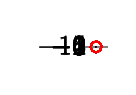
\begin{tikzpicture}

\begin{axis}[%
width=0.16\figurewidth,
height=0.16\figurewidth,
at={(0\figurewidth,0\figurewidth)},
scale only axis,
xmin=0,
xmax=1000,
xtick={\empty},
ymin=-10,
ymax=12.0029959193608,
axis background/.style={fill=white},
legend style={font=\scriptsize},
]
\addplot [color=mycolor1, forget plot]
  table[row sep=crcr]{%
1	-0.0843649488080331\\
2	-0.214008131833796\\
3	-0.679986297650323\\
4	0.305211493925368\\
5	-0.320820189309218\\
6	0.0660875607037173\\
7	-0.117371091588136\\
8	-0.291022161987253\\
9	-0.0320679252209185\\
10	-0.19145498256918\\
11	0.137546580709088\\
12	-0.787715211082825\\
13	0.308925963088189\\
14	0.840494082548609\\
15	-0.490265327250063\\
16	0.806092033427448\\
17	-0.505943733990951\\
18	0.705246702294109\\
19	-0.675181315949072\\
20	-0.458848508222575\\
21	0.982451616585212\\
22	-0.581041679167158\\
23	0.220666481524442\\
24	-0.256972343715891\\
25	0.550222935384844\\
26	0.4566084286891\\
27	-0.272822919230822\\
28	0.220816869939744\\
29	-0.558507359244571\\
30	-0.855678760268909\\
31	-0.317705845368375\\
32	-0.0942524523559566\\
33	-0.0419475645752413\\
34	0.20699547225871\\
35	0.0347572719858121\\
36	0.585373208915965\\
37	-0.821405965869159\\
38	0.167832652802413\\
39	0.364497788822494\\
40	-0.0408784048396943\\
41	0.0140846906737499\\
42	0.566618918816212\\
43	0.00300120080712023\\
44	-0.367907191656546\\
45	-0.217932304895878\\
46	-0.0497052651154481\\
47	-0.623350194236965\\
48	0.64721403859616\\
49	1.13844064451716\\
50	1.10434801033121\\
51	0.54040344646223\\
52	0.129366636868834\\
53	0.502646448028422\\
54	-0.773982262212231\\
55	0.898104936673099\\
56	0.345123854060198\\
57	0.211448090331723\\
58	-0.109884912532394\\
59	-0.56932858668193\\
60	-0.502211201390224\\
61	0.0487535691152197\\
62	0.299561132328491\\
63	0.335223708120152\\
64	-0.233822243905978\\
65	0.66348467760056\\
66	-0.486570388762728\\
67	0.0184151490386368\\
68	0.472369029086078\\
69	-0.00389672517911631\\
70	-0.641383854405865\\
71	0.963080420894394\\
72	0.548518652933385\\
73	0.798079092875706\\
74	0.494167156371459\\
75	-0.170265565219095\\
76	0.367557989586067\\
77	0.417238126503536\\
78	-0.161375393650382\\
79	0.269864268277198\\
80	0.0744945967666444\\
81	-0.0430098873828391\\
82	-0.489568370138955\\
83	-0.844125229495141\\
84	-0.785274667016293\\
85	0.466039839963624\\
86	-0.0457003485632953\\
87	0.905125252280108\\
88	-0.556547272535464\\
89	-0.617657350286978\\
90	0.0298138734677914\\
91	-1.04739822030213\\
92	0.346136444530866\\
93	-0.700436142913152\\
94	0.525530506155075\\
95	0.456183275708885\\
96	-0.805097829759135\\
97	0.0627385129567305\\
98	0.405087789518714\\
99	0.63118409272736\\
100	0.0434508866851786\\
101	-0.279905015405257\\
102	0.143067868818213\\
103	0.384466667909461\\
104	0.166942419436937\\
105	-0.139955828595503\\
106	0.0434359203402279\\
107	0.357753573332945\\
108	0.182579797183012\\
109	0.0682399944898837\\
110	-0.00311977577808928\\
111	0.451568285018243\\
112	-0.531629755675803\\
113	-0.21490694172501\\
114	0.210997955979471\\
115	-0.270089342291722\\
116	0.450421428590128\\
117	0.0873623027588145\\
118	-0.540308417520464\\
119	0.0879175754317526\\
120	0.260741702977096\\
121	-0.258503094246355\\
122	1.11995364622501\\
123	0.53550082115566\\
124	-0.359610641715548\\
125	0.468675600276672\\
126	0.792061354799461\\
127	0.135730218892354\\
128	-0.245107000332042\\
129	-0.400786564172988\\
130	-0.116550768896705\\
131	0.364376674782528\\
132	-0.122259557303792\\
133	0.0881482475513273\\
134	-0.432722586602559\\
135	-0.427543435297448\\
136	-0.657439396322772\\
137	0.175712685995699\\
138	-0.25399961572903\\
139	0.131918804460727\\
140	-0.336136413495548\\
141	-0.538389213310452\\
142	1.0316419805813\\
143	-0.524870694777161\\
144	1.0067928999215\\
145	0.631996020220941\\
146	-0.721471500555265\\
147	-0.143764802666821\\
148	-0.30567831282801\\
149	0.909544330080766\\
150	0.911541811162616\\
151	0.584249385324829\\
152	0.0295970127341896\\
153	0.74366367709583\\
154	-0.675291295179619\\
155	0.063020730591866\\
156	0.258760631640563\\
157	0.216390875482845\\
158	-0.137480747332488\\
159	-0.650287880456526\\
160	-0.276991289515375\\
161	-0.615603642656644\\
162	-0.502830163972269\\
163	1.23165373656541\\
164	-0.406350011068125\\
165	0.821326841493401\\
166	0.506211078186079\\
167	-1.27748229086424\\
168	0.383049505937469\\
169	-0.192136132483018\\
170	0.0264701801394915\\
171	0.953003193041906\\
172	0.159066791926267\\
173	-0.625485597740913\\
174	0.908080433083436\\
175	-0.240124219001492\\
176	-0.159447659055774\\
177	0.247561459400764\\
178	0.967834413535727\\
179	-0.572203461261737\\
180	0.765590457096798\\
181	0.919765433599548\\
182	-0.546265257551293\\
183	-0.275733771604057\\
184	-0.413352859087643\\
185	-0.639499401802122\\
186	-0.291994320148081\\
187	-0.28372434809682\\
188	-0.648795660661641\\
189	-0.428626798743651\\
190	-0.610926796916621\\
191	-0.482593839618813\\
192	0.426916702336307\\
193	0.323021092544632\\
194	1.12757029906748\\
195	-0.598783435496328\\
196	-0.107257163665348\\
197	0.37994115414412\\
198	-0.147932451421125\\
199	0.184947184452746\\
200	0.0955391328503245\\
201	0.0359697795547118\\
202	-0.103867461626723\\
203	-0.0993720850903125\\
204	0.432179782272863\\
205	-1.15885610496763\\
206	-0.455461620085179\\
207	0.0926504424041421\\
208	-0.394035643227185\\
209	0.968871255424605\\
210	0.287737735860074\\
211	-0.12433666179013\\
212	-0.566739182839275\\
213	-0.936631630977715\\
214	-0.04209895844447\\
215	-0.305509520899298\\
216	-0.124700133493931\\
217	0.12396380675326\\
218	0.231244530442243\\
219	-0.0849161836221947\\
220	0.514781552118051\\
221	0.382992647048255\\
222	-0.251249783634611\\
223	0.401704687956956\\
224	0.76744464382566\\
225	0.791538730227984\\
226	0.67809090567207\\
227	-0.549883178849265\\
228	-0.396629982549872\\
229	-0.156010758562395\\
230	-0.315854442308203\\
231	0.437431580142705\\
232	1.09473500820717\\
233	-0.294301079618446\\
234	-1.08299655164562\\
235	0.842062824423867\\
236	0.0736770838462823\\
237	-0.419613437613335\\
238	0.0258905249271214\\
239	0.473267396354182\\
240	-0.595386482049327\\
241	0.0509913431392351\\
242	-0.123209988684426\\
243	-0.502698721395413\\
244	0.19527896812012\\
245	-0.653678943184906\\
246	0.540246289673793\\
247	0.163753034366038\\
248	0.61012014831553\\
249	-0.670393393354344\\
250	0.0295319275262873\\
251	0.245167320991714\\
252	-1.11104383485853\\
253	0.974665342194492\\
254	0.393478495924425\\
255	-0.338995258024011\\
256	-0.00403718763406216\\
257	-0.245927454884231\\
258	-0.273764263598131\\
259	-0.027198979240364\\
260	0.201174998433531\\
261	0.0283965982299918\\
262	-0.638272144433065\\
263	-0.517500874856766\\
264	-0.506356543496489\\
265	0.182449592614664\\
266	0.175667601605455\\
267	-0.20955451674603\\
268	0.857152551769052\\
269	-1.88005915797063\\
270	0.0493606762360144\\
271	0.22161769138713\\
272	-0.78279366320501\\
273	0.17545804784859\\
274	-0.603563641501393\\
275	0.229509329763365\\
276	-0.414200788061496\\
277	-0.65483709390129\\
278	0.232357096036164\\
279	-0.470253221457708\\
280	-0.0215147013484893\\
281	-0.302289675691607\\
282	0.0285423654174946\\
283	0.209587551157584\\
284	-0.874267755727658\\
285	-0.161891194814558\\
286	-0.0363465047195934\\
287	0.782517674101749\\
288	0.623888194362764\\
289	0.334549460156666\\
290	-0.0374884151908113\\
291	-0.498684984094004\\
292	-1.00531139316928\\
293	-0.481584371736178\\
294	0.27338114648721\\
295	0.124588634449589\\
296	-0.249196538483375\\
297	0.177279386918491\\
298	-0.0414861810909713\\
299	0.212929073425452\\
300	-0.592048525773374\\
301	-0.15152106210862\\
302	-0.175201792937031\\
303	0.361616786525534\\
304	-0.582984577965842\\
305	-1.08940111252282\\
306	-0.719244760295982\\
307	1.08250996178419\\
308	0.0998609794011087\\
309	0.360734067689575\\
310	0.637360529423789\\
311	0.175104013890239\\
312	-0.0667266377332547\\
313	-0.578488741131812\\
314	0.584724778956588\\
315	0.596210312215142\\
316	0.125109426992008\\
317	-0.51845734338376\\
318	0.108804573787487\\
319	-0.259539016571146\\
320	0.810137518496697\\
321	-0.383656593991318\\
322	-0.522407748663148\\
323	0.503978373243993\\
324	-0.243567345359413\\
325	-1.172990068322\\
326	-0.22198782989142\\
327	-0.0615399881163718\\
328	0.48798850215915\\
329	0.507531758342685\\
330	-0.306642722479194\\
331	-0.423625983080607\\
332	0.166597166251104\\
333	0.448928558608505\\
334	0.556639083785501\\
335	0.192140699909011\\
336	-0.0095516640157447\\
337	-0.303453170566988\\
338	-0.225262668235192\\
339	-0.170966602416872\\
340	-0.0695753821512942\\
341	-0.340825151996071\\
342	-0.978947487802297\\
343	-0.226396155987391\\
344	-0.511181837946741\\
345	0.884286011861108\\
346	-0.644406311863771\\
347	0.0995456810527316\\
348	0.0642815174838746\\
349	0.458824247936378\\
350	0.610466405880688\\
351	0.35329175155191\\
352	0.00919178943440044\\
353	-0.582928674508939\\
354	0.444169718553649\\
355	0.81661795815895\\
356	0.117847659547683\\
357	1.10228320155493\\
358	0.21237503754539\\
359	-0.331252871246226\\
360	0.0190174614596223\\
361	-0.326825487724887\\
362	0.543086025273431\\
363	-0.273505612924781\\
364	0.403132767171386\\
365	-0.00414979160048917\\
366	0.0672107732096745\\
367	0.719439879980519\\
368	0.0855164761467874\\
369	-1.14137795872991\\
370	0.472856962692473\\
371	0.0528272322242862\\
372	0.0587772697395647\\
373	0.312734399046126\\
374	-0.00829142713004922\\
375	-0.0463189601597944\\
376	0.144497131102709\\
377	-0.914612347698413\\
378	0.0656516802165435\\
379	0.254362724299455\\
380	0.492259401102319\\
381	-0.606505952498766\\
382	0.417462854205637\\
383	-0.592271173104314\\
384	-0.0800123698641439\\
385	0.0360006062423074\\
386	0.944791948424782\\
387	0.0321696046755821\\
388	1.11836201649462\\
389	-0.599042331906903\\
390	-0.320916358041544\\
391	-0.165931798872961\\
392	0.376716644185482\\
393	0.270834176287245\\
394	0.97620901718682\\
395	0.577946898388241\\
396	-0.176054363783005\\
397	0.504272077962293\\
398	0.761622013597124\\
399	-0.305588317768251\\
400	0.378369582481294\\
401	-0.225836896993232\\
402	-0.341511344655298\\
403	-0.588938065886378\\
404	-0.159382870110183\\
405	0.599466724419285\\
406	0.631870899036544\\
407	0.569968379702726\\
408	0.449221508660479\\
409	0.254247886154118\\
410	-0.227546553200521\\
411	0.189183538362055\\
412	0.0103502906884314\\
413	-0.298128218012405\\
414	0.466264400800278\\
415	-0.297841375071721\\
416	-0.363090798260781\\
417	-0.805201179687854\\
418	0.618903899477659\\
419	-0.241505299002811\\
420	0.195885248007496\\
421	-0.00392323024707546\\
422	0.151391554166215\\
423	-1.05722679473409\\
424	0.641613532277937\\
425	-0.425708645245871\\
426	-0.317355253145289\\
427	0.277295763226701\\
428	0.295488729296796\\
429	0.0136578849953828\\
430	-0.756828466438818\\
431	-0.33253001138564\\
432	0.0885166086385254\\
433	0.0806404792175083\\
434	0.102049489820487\\
435	0.161488641149125\\
436	-0.531260107577739\\
437	0.64175481248038\\
438	0.51387975143736\\
439	-0.00180619830304196\\
440	-0.611733455639115\\
441	-0.561487753860683\\
442	0.000622488470140382\\
443	-0.365579588851063\\
444	0.713597266355123\\
445	0.258631227865919\\
446	-0.515499059857584\\
447	-0.387954901719725\\
448	-0.185691221388841\\
449	-0.49737564505894\\
450	-0.127698960372597\\
451	0.821258306094292\\
452	-0.603960405096216\\
453	0.303860583598852\\
454	-0.755012092630766\\
455	-0.405655716431988\\
456	-0.116403541633505\\
457	0.661744538224954\\
458	-0.158841769759258\\
459	0.187953018977439\\
460	0.545823105842562\\
461	0.0171988424159846\\
462	0.189635796204109\\
463	-0.0744054376638616\\
464	-0.21401907043828\\
465	-0.433284104339181\\
466	0.67883729311031\\
467	-0.291836355195805\\
468	-0.213327794769529\\
469	-0.749160298177028\\
470	0.286410094610351\\
471	0.140656287027374\\
472	1.13898821825384\\
473	-0.169352442397022\\
474	-0.0307120991469569\\
475	0.0276262598982887\\
476	0.224852089179212\\
477	0.739445433813322\\
478	-0.618331027742564\\
479	-0.657953344356246\\
480	-0.19473040509835\\
481	-0.425795273242851\\
482	-0.072914825182719\\
483	-0.0696173668585981\\
484	0.376074255655421\\
485	0.0653390574113868\\
486	0.645984790107609\\
487	-0.586809336424126\\
488	-0.166379973131452\\
489	-0.275758044911234\\
490	0.78439378620984\\
491	-0.0361746646653177\\
492	-1.00214431449453\\
493	0.27774844240369\\
494	0.0806686064168886\\
495	-0.0627020077389101\\
496	-0.289053258558686\\
497	0.676637374553753\\
498	-0.00720306095510542\\
499	-1.06165919816529\\
500	0.68472074565485\\
501	-0.133806778147483\\
502	-0.179134532826954\\
503	0.529240886120155\\
504	0.0590518326672562\\
505	0.570312420474795\\
506	0.338843933062209\\
507	0.172575858493757\\
508	-0.504569703121305\\
509	0.685555937861077\\
510	0.131259434042635\\
511	-0.176498177899002\\
512	0.309839521019899\\
513	0.121702142710417\\
514	-0.100632042470991\\
515	0.655600122753057\\
516	-0.235030982211496\\
517	-0.679298044018366\\
518	0.534766095616803\\
519	-0.0567688143745623\\
520	-0.370972412808836\\
521	0.157956465354228\\
522	0.132416252413451\\
523	-0.243931746381284\\
524	-0.192000895427328\\
525	-0.72637556961118\\
526	-0.595884584865918\\
527	-0.218212475142704\\
528	-0.552098290621037\\
529	-0.272320318324217\\
530	-0.171960456782646\\
531	0.00181018410387911\\
532	-0.336669630665833\\
533	0.0161834272880342\\
534	0.395954314133312\\
535	-0.250729398499196\\
536	0.543109549027052\\
537	0.781167845648345\\
538	-0.448854884656915\\
539	-0.0199998129557289\\
540	-0.320551008581919\\
541	-0.669622257360215\\
542	-0.38885088871067\\
543	0.389757946917205\\
544	-0.162656202823606\\
545	0.313876620675959\\
546	-0.146974311208132\\
547	0.237789207587749\\
548	-0.435832122572481\\
549	-0.674044795282498\\
550	0.529063700919542\\
551	-0.336567799102003\\
552	-0.204452769291567\\
553	0.613472182402155\\
554	-0.528679561447113\\
555	-0.480345143573817\\
556	-0.279765349349785\\
557	0.70368446421643\\
558	0.207203925649419\\
559	-0.702309716931273\\
560	-0.0821962799919988\\
561	-0.0226548302528977\\
562	0.10419443516641\\
563	-0.370455616466144\\
564	0.0246043794246438\\
565	-0.273259999629885\\
566	-0.17896780103803\\
567	0.106680226526235\\
568	-0.85531217642154\\
569	0.355811011811776\\
570	-0.566214111855081\\
571	-0.486719885126287\\
572	0.0427086365930212\\
573	0.0419673984856579\\
574	0.210082313599684\\
575	0.0417057668187157\\
576	0.323535363254175\\
577	-0.400615366176869\\
578	0.0183512757531864\\
579	0.366913853449974\\
580	-0.553390224026931\\
581	0.994101733510469\\
582	0.100222675982646\\
583	-0.310729371702411\\
584	-0.698388665782107\\
585	0.363125967960498\\
586	-0.142337430554337\\
587	-0.443986445786511\\
588	0.718235737371446\\
589	-0.603949680483409\\
590	1.25938859595364\\
591	0.559454286224595\\
592	0.270354433528082\\
593	0.21987374019503\\
594	0.156611320651543\\
595	-1.070333599805\\
596	-0.116363819298723\\
597	-0.19933830592858\\
598	0.633760914960439\\
599	-0.422601919910047\\
600	-0.199245082064498\\
601	0.416645859600199\\
602	-0.70579918757247\\
603	-1.308605970333\\
604	-0.184548420998238\\
605	0.648355322844126\\
606	-0.297172285068241\\
607	0.370624280956993\\
608	-0.178097620075753\\
609	0.159281889738392\\
610	-0.12071671423136\\
611	0.528014335571112\\
612	0.406091489869186\\
613	0.371243145572002\\
614	-0.704066137984947\\
615	-0.644245413407105\\
616	-0.242582657737263\\
617	-0.29827686603773\\
618	0.0164902521183513\\
619	0.581106839611111\\
620	-0.352007792348193\\
621	0.173377867046313\\
622	-0.0727527818909391\\
623	0.222494399075518\\
624	0.0728142510928137\\
625	-0.187844494335508\\
626	0.117964592612995\\
627	-0.610339422666212\\
628	-0.299935450901594\\
629	-0.0010706315983897\\
630	-0.564701709138396\\
631	-0.507179068710608\\
632	0.0877700636655975\\
633	-0.229508906857061\\
634	0.308990747891106\\
635	-0.724348580612654\\
636	-0.274295267031075\\
637	-0.395720013258778\\
638	0.753230590460362\\
639	0.233876511406342\\
640	0.0184357279760769\\
641	-1.10274386929427\\
642	-0.318548755099341\\
643	0.517053427718337\\
644	-0.902730414325686\\
645	-0.409743253222495\\
646	0.969226042438119\\
647	0.258259973527672\\
648	1.11515300947101\\
649	-0.367191232730355\\
650	0.554106606252066\\
651	-0.379917299422178\\
652	-0.666986539838205\\
653	-0.345171256055159\\
654	-9.76884855107274e-05\\
655	-0.472212088412179\\
656	-0.333295799842747\\
657	-0.16945779352062\\
658	-0.305713981548694\\
659	0.610687848132281\\
660	0.417522591912876\\
661	1.07455865476785\\
662	-0.203058711118244\\
663	-0.167481546669517\\
664	0.893310263567852\\
665	0.199358121273893\\
666	-0.229482628269498\\
667	0.257167172771096\\
668	0.785269226723262\\
669	-1.10456606880831\\
670	0.398083768245946\\
671	0.0564197000422718\\
672	0.00243736604964581\\
673	0.143384976503503\\
674	-0.123046601679984\\
675	0.777155096915594\\
676	-0.764606137269861\\
677	0.555100530389379\\
678	0.139816738775491\\
679	-0.725082920654946\\
680	0.0680025729938574\\
681	0.396726972569839\\
682	-0.359327827218925\\
683	0.653784362486646\\
684	0.0982515809232709\\
685	-0.542960006727409\\
686	0.523313929544635\\
687	-0.156390201987887\\
688	0.246662543170651\\
689	-0.233340723909457\\
690	0.00401667108651162\\
691	-0.610022273056647\\
692	-1.13772708672788\\
693	0.0709084479363042\\
694	0.736185051964045\\
695	0.160149839955152\\
696	-0.014087981202213\\
697	0.197719144781034\\
698	0.309645827956685\\
699	-1.23394702325022\\
700	-0.0919258488852546\\
701	-0.962880866882831\\
702	0.100974258796012\\
703	-0.131721327988481\\
704	-0.819127812270075\\
705	1.20490280007633\\
706	-0.477654916251542\\
707	-0.500021741977231\\
708	0.23600999574695\\
709	0.0374396552269687\\
710	0.123498289224641\\
711	-0.0354103433000551\\
712	-0.217221375384679\\
713	0.38653067115683\\
714	-0.0249848903850201\\
715	0.291875632093308\\
716	-1.00130582015446\\
717	0.0647356255097095\\
718	-0.890244841129502\\
719	-0.271989210178287\\
720	-0.394545347840677\\
721	-0.28803784752075\\
722	-1.08696007899737\\
723	-0.668112507662126\\
724	0.0930311022388154\\
725	-0.0813004903091181\\
726	0.757064172304368\\
727	0.913437969258064\\
728	0.507335455346513\\
729	0.388960581710665\\
730	0.434494218265819\\
731	0.094068283768907\\
732	0.0776779117524501\\
733	0.433621845589042\\
734	0.00476580511195274\\
735	0.11661910996473\\
736	-0.235404725283676\\
737	-0.279578464873324\\
738	-1.19772285900132\\
739	-0.374986056851166\\
740	-0.0634462158626879\\
741	-0.205277250607372\\
742	0.0360768546541328\\
743	0.0344357765964842\\
744	0.465051980363597\\
745	-0.32005920079798\\
746	0.753105384577899\\
747	-0.16340667665109\\
748	-0.0584263265639761\\
749	-0.178591335959003\\
750	0.225988342060698\\
751	0.0744459928684163\\
752	0.0656673158543383\\
753	0.031584515859645\\
754	-0.00116915865028563\\
755	-0.161232958257285\\
756	0.0803582785930206\\
757	-0.15218490047797\\
758	0.188699101523886\\
759	0.0176253797464635\\
760	-0.127603999537356\\
761	0.207131952978449\\
762	0.244210881527307\\
763	-0.0435989053169047\\
764	-0.281776952406611\\
765	0.209745128466236\\
766	-0.234897065766475\\
767	-0.802847662483007\\
768	0.108335817639795\\
769	0.293532501880131\\
770	-1.20657701467902\\
771	-0.324697984241396\\
772	-0.871792673559817\\
773	0.147171106130246\\
774	0.0418698096961806\\
775	0.296498656828848\\
776	0.651976777003359\\
777	-0.374581482199088\\
778	0.287391773120637\\
779	-0.487923194516853\\
780	0.484070989230847\\
781	-0.0652064094233195\\
782	-0.107377900772722\\
783	-0.548403228877828\\
784	-0.304592186756698\\
785	-0.138786969972267\\
786	-0.480064011054402\\
787	-0.911246716447289\\
788	1.02618485745961\\
789	0.284816576207211\\
790	0.166984038661823\\
791	-0.272037953635982\\
792	-0.42714616220688\\
793	-0.625979187443832\\
794	-0.391617221617088\\
795	-0.06306395390893\\
796	0.145452779188216\\
797	0.151310995006072\\
798	-0.218771197636809\\
799	0.558499974948029\\
800	-0.695246089677069\\
801	-1.19066285359777\\
802	0.405738135779963\\
803	-0.212229618151057\\
804	-0.872377312813768\\
805	-0.575433800061526\\
806	0.15582119223586\\
807	0.447772543974477\\
808	-0.224348121904101\\
809	0.674941557740976\\
810	0.382939125080821\\
811	-0.14800620883972\\
812	-0.815402420989961\\
813	-0.488729938619766\\
814	0.75803385924224\\
815	0.828844203597021\\
816	-0.185620175534317\\
817	0.0466039499913011\\
818	-0.759764467270089\\
819	0.191421034604269\\
820	0.262880328813764\\
821	-0.305585094795894\\
822	-0.236822193646006\\
823	-0.14222534654938\\
824	0.0190925766660391\\
825	0.300889850804001\\
826	0.409484177727915\\
827	-0.156809450679849\\
828	-0.310896513052183\\
829	0.999211997378169\\
830	0.225798882134653\\
831	0.748393882440885\\
832	-0.593339077066278\\
833	0.284555270958646\\
834	0.794943889138576\\
835	-0.509337960187581\\
836	0.188143758717045\\
837	0.136868150798884\\
838	0.124820337466264\\
839	-0.40888113709964\\
840	-0.479369161157232\\
841	-0.445547660040124\\
842	-0.443001364533436\\
843	-0.862653050522362\\
844	-0.2907755201939\\
845	-0.897156925960066\\
846	0.124447259778338\\
847	0.388208673924113\\
848	0.821622864053029\\
849	-0.655955540940912\\
850	-0.272573496562315\\
851	0.97783752911077\\
852	0.774041279034294\\
853	0.463500727683254\\
854	0.109283871279626\\
855	-0.259951771334581\\
856	0.424542384229059\\
857	0.714796287430657\\
858	-0.606746592462782\\
859	0.0970094479335378\\
860	0.483500913970844\\
861	-0.146567802800952\\
862	-0.0201208882048664\\
863	-0.311812744609704\\
864	1.49015256382447\\
865	-0.444626029395034\\
866	0.824370395084279\\
867	0.780561835745967\\
868	-0.66535664481576\\
869	-0.0658559309614565\\
870	-0.0573171983676417\\
871	0.514668452128276\\
872	-0.100134431673895\\
873	-1.22316772178064\\
874	1.03601477062912\\
875	-0.107887886329332\\
876	-0.501540075349896\\
877	-0.866350837438675\\
878	0.175457801139091\\
879	0.675007607890228\\
880	0.738554381372377\\
881	-0.465359594803733\\
882	-0.208048420858485\\
883	-0.172617597165389\\
884	-0.185023041192956\\
885	-0.397382185710709\\
886	-0.0729763660209233\\
887	0.407156938601771\\
888	-0.0212416689994082\\
889	-0.898715359753816\\
890	0.36602645333211\\
891	-0.00309765391866012\\
892	0.164674708306813\\
893	0.351348971757383\\
894	0.162369819639995\\
895	-0.392762533370197\\
896	0.301244442757363\\
897	-0.108310529208443\\
898	-0.226510575558495\\
899	-0.0543052860725728\\
900	0.506042251221722\\
901	0.576467121819494\\
902	0.640473156676736\\
903	-0.0271484031789434\\
904	-0.44903587703174\\
905	-0.139874583767367\\
906	-0.323418721715264\\
907	-0.224017872627231\\
908	-0.404715682262724\\
909	-0.323598838181954\\
910	-0.720544148648756\\
911	-0.446693661968103\\
912	-0.352280510858124\\
913	0.89106955607507\\
914	-0.0269839249507989\\
915	-0.886399859448943\\
916	0.329879606552847\\
917	-0.830450089259012\\
918	-0.0303319147082194\\
919	0.438917745217486\\
920	-1.03407915688438\\
921	-0.148705435094169\\
922	0.0750143952964256\\
923	0.183290234160649\\
924	-0.301622618467814\\
925	-0.0291096649336722\\
926	0.455121903062052\\
927	0.634519778664822\\
928	0.237354698668951\\
929	0.395328635159354\\
930	0.0874987304801428\\
931	-0.0739094280762626\\
932	1.1348044252952\\
933	-1.00552338142747\\
934	-0.464424408604261\\
935	0.398693399939488\\
936	-0.157464360454095\\
937	0.170514924677735\\
938	0.150914113616135\\
939	0.0102741063303847\\
940	-0.246832089564145\\
941	0.208525738405877\\
942	-0.933584226680535\\
943	-0.801580228955027\\
944	-0.738673600457794\\
945	0.537233562652825\\
946	-0.466287278102476\\
947	0.337162488538628\\
948	0.68517391558206\\
949	-0.363056496910801\\
950	-0.0702136894923856\\
951	-0.413399287696376\\
952	-0.955385968653268\\
953	-0.0809817275933897\\
954	0.759452154277243\\
955	0.142166691752978\\
956	0.283794098072679\\
957	0.41612317065253\\
958	-0.255698807862619\\
959	-0.289183729896512\\
960	0.0117181104555458\\
961	-0.946983620103819\\
962	0.550071777194288\\
963	-0.382902468847065\\
964	0.242257451056003\\
965	0.0445267970424669\\
966	1.02035597314192\\
967	0.201733006766947\\
968	0.526610799396121\\
969	-0.0727116911297317\\
970	-0.797221053581196\\
971	-0.0434892243892349\\
972	-1.22702964906741\\
973	-0.62422509950225\\
974	-0.239074815579112\\
975	0.254134345530693\\
976	-0.400344706072007\\
977	0.0454306875166548\\
978	-0.0308610513642432\\
979	0.0355528628733202\\
980	-0.0479653544291591\\
981	0.802270628620476\\
982	0.283042884646343\\
983	0.0732231666950477\\
984	0.712274578803625\\
985	0.390894932457267\\
986	-0.479115001951279\\
987	-0.615600855930176\\
988	-1.46840564254481\\
989	-0.381511586944676\\
990	0.0183820748192244\\
991	-0.851869668016771\\
992	-0.693127380571038\\
993	-0.279778847149423\\
994	-0.183743838770135\\
995	0.605819709300724\\
996	0.143707092762505\\
997	-1.37801050970886\\
998	0.580021716861414\\
999	-0.325143928421166\\
1000	0.470756034388443\\
};
\addplot [color=mycolor2, dotted, forget plot]
  table[row sep=crcr]{%
1	-0.0843649488080331\\
2	-0.214008131833796\\
3	-0.679986297650323\\
4	0.305211493925368\\
5	-0.320820189309218\\
6	0.0660875607037173\\
7	-0.117371091588136\\
8	-0.291022161987253\\
9	-0.0320679252209185\\
10	-0.19145498256918\\
11	0.137546580709088\\
12	-0.787715211082825\\
13	0.308925963088189\\
14	0.840494082548609\\
15	-0.490265327250063\\
16	0.806092033427448\\
17	-0.505943733990951\\
18	0.705246702294109\\
19	-0.675181315949072\\
20	-0.458848508222575\\
21	0.982451616585212\\
22	-0.581041679167158\\
23	0.220666481524442\\
24	-0.256972343715891\\
25	0.550222935384844\\
26	0.4566084286891\\
27	-0.272822919230822\\
28	0.220816869939744\\
29	-0.558507359244571\\
30	-0.855678760268909\\
31	-0.317705845368375\\
32	-0.0942524523559566\\
33	-0.0419475645752413\\
34	0.20699547225871\\
35	0.0347572719858121\\
36	0.585373208915965\\
37	-0.821405965869159\\
38	0.167832652802413\\
39	0.364497788822494\\
40	-0.0408784048396943\\
41	0.0140846906737499\\
42	0.566618918816212\\
43	0.00300120080712023\\
44	-0.367907191656546\\
45	-0.217932304895878\\
46	-0.0497052651154481\\
47	-0.623350194236965\\
48	0.64721403859616\\
49	1.13844064451716\\
50	1.10434801033121\\
51	0.54040344646223\\
52	0.129366636868834\\
53	0.502646448028422\\
54	-0.773982262212231\\
55	0.898104936673099\\
56	0.345123854060198\\
57	0.211448090331723\\
58	-0.109884912532394\\
59	-0.56932858668193\\
60	-0.502211201390224\\
61	0.0487535691152197\\
62	0.299561132328491\\
63	3.06646637935014\\
64	-0.233822243905978\\
65	0.66348467760056\\
66	-0.486570388762728\\
67	0.0184151490386368\\
68	0.472369029086078\\
69	-0.00389672517911631\\
70	-0.641383854405865\\
71	0.963080420894394\\
72	0.548518652933385\\
73	0.798079092875706\\
74	0.494167156371459\\
75	-0.170265565219095\\
76	0.367557989586067\\
77	0.417238126503536\\
78	-0.161375393650382\\
79	0.269864268277198\\
80	0.0744945967666444\\
81	-0.0430098873828391\\
82	-0.489568370138955\\
83	-0.844125229495141\\
84	-0.785274667016293\\
85	0.466039839963624\\
86	-0.0457003485632953\\
87	0.905125252280108\\
88	-0.556547272535464\\
89	-0.617657350286978\\
90	0.0298138734677914\\
91	-1.04739822030213\\
92	0.346136444530866\\
93	-0.700436142913152\\
94	0.525530506155075\\
95	0.456183275708885\\
96	-0.805097829759135\\
97	0.0627385129567305\\
98	0.405087789518714\\
99	0.63118409272736\\
100	0.0434508866851786\\
101	-0.279905015405257\\
102	0.143067868818213\\
103	0.384466667909461\\
104	0.166942419436937\\
105	-0.139955828595503\\
106	0.0434359203402279\\
107	0.357753573332945\\
108	0.182579797183012\\
109	0.0682399944898837\\
110	-0.00311977577808928\\
111	0.451568285018243\\
112	-0.531629755675803\\
113	0.0510025608660534\\
114	0.210997955979471\\
115	-0.270089342291722\\
116	-2.16887249520696\\
117	0.0873623027588145\\
118	-0.540308417520464\\
119	0.0879175754317526\\
120	0.260741702977096\\
121	-0.258503094246355\\
122	1.11995364622501\\
123	0.53550082115566\\
124	-0.359610641715548\\
125	0.468675600276672\\
126	0.792061354799461\\
127	0.135730218892354\\
128	-0.245107000332042\\
129	-0.400786564172988\\
130	-0.116550768896705\\
131	0.364376674782528\\
132	-0.122259557303792\\
133	0.0881482475513273\\
134	-0.432722586602559\\
135	-0.427543435297448\\
136	-0.657439396322772\\
137	0.175712685995699\\
138	-0.25399961572903\\
139	0.131918804460727\\
140	-0.336136413495548\\
141	-0.538389213310452\\
142	1.0316419805813\\
143	-0.524870694777161\\
144	1.0067928999215\\
145	0.631996020220941\\
146	-0.721471500555265\\
147	-0.143764802666821\\
148	-0.30567831282801\\
149	0.909544330080766\\
150	0.911541811162616\\
151	0.584249385324829\\
152	0.0295970127341896\\
153	0.74366367709583\\
154	-0.675291295179619\\
155	0.063020730591866\\
156	0.258760631640563\\
157	0.216390875482845\\
158	-0.137480747332488\\
159	-0.650287880456526\\
160	-0.276991289515375\\
161	-0.615603642656644\\
162	-0.502830163972269\\
163	1.23165373656541\\
164	-0.406350011068125\\
165	0.821326841493401\\
166	0.506211078186079\\
167	-1.27748229086424\\
168	0.383049505937469\\
169	-0.192136132483018\\
170	0.0264701801394915\\
171	0.953003193041906\\
172	0.159066791926267\\
173	-0.625485597740913\\
174	0.908080433083436\\
175	-0.240124219001492\\
176	-0.159447659055774\\
177	0.247561459400764\\
178	0.967834413535727\\
179	-0.572203461261737\\
180	0.765590457096798\\
181	0.919765433599548\\
182	-0.546265257551293\\
183	-0.275733771604057\\
184	-0.413352859087643\\
185	-0.639499401802122\\
186	-0.291994320148081\\
187	-0.28372434809682\\
188	-0.648795660661641\\
189	-0.428626798743651\\
190	-0.610926796916621\\
191	-0.482593839618813\\
192	0.426916702336307\\
193	0.323021092544632\\
194	1.12757029906748\\
195	-0.598783435496328\\
196	-0.107257163665348\\
197	0.37994115414412\\
198	-0.147932451421125\\
199	0.184947184452746\\
200	0.0955391328503245\\
201	0.0359697795547118\\
202	0.446274309422204\\
203	-0.0993720850903125\\
204	0.432179782272863\\
205	-1.15885610496763\\
206	-0.455461620085179\\
207	0.0926504424041421\\
208	-0.394035643227185\\
209	0.968871255424605\\
210	0.287737735860074\\
211	-0.12433666179013\\
212	2.58539635186793\\
213	-0.936631630977715\\
214	-0.04209895844447\\
215	-0.305509520899298\\
216	-0.124700133493931\\
217	0.12396380675326\\
218	0.231244530442243\\
219	-0.0849161836221947\\
220	0.514781552118051\\
221	0.382992647048255\\
222	-0.251249783634611\\
223	0.401704687956956\\
224	0.76744464382566\\
225	0.791538730227984\\
226	0.67809090567207\\
227	-0.549883178849265\\
228	-0.396629982549872\\
229	-0.156010758562395\\
230	-0.315854442308203\\
231	0.437431580142705\\
232	1.09473500820717\\
233	-0.294301079618446\\
234	-1.08299655164562\\
235	0.842062824423867\\
236	0.0736770838462823\\
237	-0.419613437613335\\
238	0.0258905249271214\\
239	0.473267396354182\\
240	-0.595386482049327\\
241	0.0509913431392351\\
242	-0.123209988684426\\
243	-0.502698721395413\\
244	0.19527896812012\\
245	-0.653678943184906\\
246	0.540246289673793\\
247	0.163753034366038\\
248	0.61012014831553\\
249	-0.670393393354344\\
250	0.0295319275262873\\
251	0.245167320991714\\
252	-1.11104383485853\\
253	0.974665342194492\\
254	0.393478495924425\\
255	-0.338995258024011\\
256	-0.00403718763406216\\
257	-0.245927454884231\\
258	-0.273764263598131\\
259	-0.027198979240364\\
260	0.201174998433531\\
261	0.0283965982299918\\
262	-0.638272144433065\\
263	-0.517500874856766\\
264	-0.506356543496489\\
265	0.182449592614664\\
266	0.175667601605455\\
267	0.949018073307561\\
268	0.857152551769052\\
269	-1.88005915797063\\
270	-0.156067424066943\\
271	0.22161769138713\\
272	-0.78279366320501\\
273	0.17545804784859\\
274	-0.603563641501393\\
275	0.229509329763365\\
276	-0.414200788061496\\
277	-0.65483709390129\\
278	0.232357096036164\\
279	-0.470253221457708\\
280	-0.0215147013484893\\
281	0.333094008977015\\
282	0.0285423654174946\\
283	0.209587551157584\\
284	-0.874267755727658\\
285	-0.161891194814558\\
286	-0.0363465047195934\\
287	0.782517674101749\\
288	0.623888194362764\\
289	0.334549460156666\\
290	-0.0374884151908113\\
291	-0.498684984094004\\
292	-1.00531139316928\\
293	-0.481584371736178\\
294	0.27338114648721\\
295	0.124588634449589\\
296	-0.249196538483375\\
297	0.177279386918491\\
298	-0.0414861810909713\\
299	0.212929073425452\\
300	-0.592048525773374\\
301	-0.15152106210862\\
302	-0.175201792937031\\
303	0.361616786525534\\
304	-0.582984577965842\\
305	-1.08940111252282\\
306	-0.719244760295982\\
307	1.08250996178419\\
308	0.0998609794011087\\
309	0.360734067689575\\
310	0.637360529423789\\
311	0.175104013890239\\
312	-0.0667266377332547\\
313	-0.578488741131812\\
314	0.584724778956588\\
315	0.596210312215142\\
316	0.125109426992008\\
317	-0.51845734338376\\
318	0.108804573787487\\
319	-0.259539016571146\\
320	0.810137518496697\\
321	-0.383656593991318\\
322	-0.522407748663148\\
323	0.503978373243993\\
324	-0.243567345359413\\
325	-1.172990068322\\
326	-0.22198782989142\\
327	-0.0615399881163718\\
328	0.48798850215915\\
329	0.507531758342685\\
330	-0.306642722479194\\
331	-0.423625983080607\\
332	0.166597166251104\\
333	0.448928558608505\\
334	0.556639083785501\\
335	0.192140699909011\\
336	-0.0095516640157447\\
337	-0.303453170566988\\
338	-0.225262668235192\\
339	-0.170966602416872\\
340	-0.0695753821512942\\
341	-0.340825151996071\\
342	-0.978947487802297\\
343	-0.226396155987391\\
344	-0.511181837946741\\
345	0.884286011861108\\
346	-0.644406311863771\\
347	0.0995456810527316\\
348	0.0642815174838746\\
349	0.458824247936378\\
350	0.610466405880688\\
351	0.35329175155191\\
352	0.00919178943440044\\
353	-0.582928674508939\\
354	0.444169718553649\\
355	0.81661795815895\\
356	0.117847659547683\\
357	1.10228320155493\\
358	0.21237503754539\\
359	-0.331252871246226\\
360	0.0190174614596223\\
361	1.17814360194014\\
362	0.543086025273431\\
363	-0.273505612924781\\
364	0.403132767171386\\
365	-0.00414979160048917\\
366	0.0672107732096745\\
367	0.719439879980519\\
368	0.0855164761467874\\
369	-1.14137795872991\\
370	0.472856962692473\\
371	0.0528272322242862\\
372	0.0587772697395647\\
373	0.312734399046126\\
374	-0.00829142713004922\\
375	-0.0463189601597944\\
376	0.144497131102709\\
377	-0.914612347698413\\
378	0.0656516802165435\\
379	0.254362724299455\\
380	0.492259401102319\\
381	-0.606505952498766\\
382	0.417462854205637\\
383	-0.592271173104314\\
384	-0.0800123698641439\\
385	0.0360006062423074\\
386	0.944791948424782\\
387	0.0321696046755821\\
388	1.11836201649462\\
389	-0.599042331906903\\
390	-0.320916358041544\\
391	-0.165931798872961\\
392	0.376716644185482\\
393	0.270834176287245\\
394	0.97620901718682\\
395	0.577946898388241\\
396	-0.176054363783005\\
397	0.504272077962293\\
398	0.761622013597124\\
399	-0.305588317768251\\
400	0.378369582481294\\
401	-0.225836896993232\\
402	-0.341511344655298\\
403	-0.588938065886378\\
404	-0.159382870110183\\
405	0.599466724419285\\
406	0.631870899036544\\
407	0.569968379702726\\
408	0.449221508660479\\
409	0.254247886154118\\
410	-0.227546553200521\\
411	0.189183538362055\\
412	0.0103502906884314\\
413	-0.298128218012405\\
414	0.466264400800278\\
415	-0.297841375071721\\
416	-0.363090798260781\\
417	-0.805201179687854\\
418	-3.25868400722303\\
419	-0.241505299002811\\
420	0.195885248007496\\
421	-0.00392323024707546\\
422	0.151391554166215\\
423	-1.05722679473409\\
424	0.641613532277937\\
425	-0.425708645245871\\
426	-0.317355253145289\\
427	0.277295763226701\\
428	0.295488729296796\\
429	0.0136578849953828\\
430	-0.756828466438818\\
431	-0.33253001138564\\
432	0.0885166086385254\\
433	0.0806404792175083\\
434	0.102049489820487\\
435	0.161488641149125\\
436	-0.531260107577739\\
437	0.64175481248038\\
438	0.51387975143736\\
439	-0.0106691835205184\\
440	-0.611733455639115\\
441	-0.561487753860683\\
442	0.000622488470140382\\
443	-0.365579588851063\\
444	0.713597266355123\\
445	0.258631227865919\\
446	-0.515499059857584\\
447	-0.387954901719725\\
448	-0.185691221388841\\
449	-0.49737564505894\\
450	-0.127698960372597\\
451	0.821258306094292\\
452	-0.603960405096216\\
453	0.303860583598852\\
454	-0.755012092630766\\
455	-0.405655716431988\\
456	-0.116403541633505\\
457	0.661744538224954\\
458	-0.43755531272699\\
459	0.187953018977439\\
460	0.545823105842562\\
461	0.0171988424159846\\
462	0.189635796204109\\
463	-0.0744054376638616\\
464	-0.21401907043828\\
465	-0.433284104339181\\
466	0.67883729311031\\
467	-0.291836355195805\\
468	-0.213327794769529\\
469	-0.749160298177028\\
470	2.19486074087304\\
471	0.140656287027374\\
472	1.13898821825384\\
473	-0.169352442397022\\
474	-0.0307120991469569\\
475	0.0276262598982887\\
476	0.224852089179212\\
477	0.739445433813322\\
478	-0.618331027742564\\
479	-0.657953344356246\\
480	-0.19473040509835\\
481	-0.425795273242851\\
482	-0.072914825182719\\
483	-0.0696173668585981\\
484	0.376074255655421\\
485	0.0653390574113868\\
486	0.645984790107609\\
487	-0.586809336424126\\
488	-0.166379973131452\\
489	-0.275758044911234\\
490	0.78439378620984\\
491	-0.0361746646653177\\
492	-1.00214431449453\\
493	0.27774844240369\\
494	0.0806686064168886\\
495	-0.0627020077389101\\
496	-0.289053258558686\\
497	0.676637374553753\\
498	-0.00720306095510542\\
499	-1.06165919816529\\
500	0.68472074565485\\
501	-0.133806778147483\\
502	-0.179134532826954\\
503	0.529240886120155\\
504	0.0590518326672562\\
505	0.570312420474795\\
506	0.338843933062209\\
507	0.172575858493757\\
508	-0.504569703121305\\
509	0.685555937861077\\
510	0.131259434042635\\
511	-0.176498177899002\\
512	0.309839521019899\\
513	0.121702142710417\\
514	-0.100632042470991\\
515	0.655600122753057\\
516	-0.235030982211496\\
517	-0.679298044018366\\
518	0.534766095616803\\
519	-0.0567688143745623\\
520	-0.370972412808836\\
521	0.157956465354228\\
522	0.132416252413451\\
523	-0.243931746381284\\
524	-0.192000895427328\\
525	-0.72637556961118\\
526	-0.595884584865918\\
527	-0.218212475142704\\
528	-0.552098290621037\\
529	-0.272320318324217\\
530	-0.171960456782646\\
531	0.00181018410387911\\
532	-0.336669630665833\\
533	0.0161834272880342\\
534	0.395954314133312\\
535	-0.250729398499196\\
536	0.543109549027052\\
537	0.781167845648345\\
538	-0.448854884656915\\
539	-0.0199998129557289\\
540	-0.320551008581919\\
541	-0.669622257360215\\
542	-0.38885088871067\\
543	0.389757946917205\\
544	-0.162656202823606\\
545	0.313876620675959\\
546	-0.146974311208132\\
547	0.237789207587749\\
548	-0.435832122572481\\
549	-0.674044795282498\\
550	0.529063700919542\\
551	-0.336567799102003\\
552	-0.204452769291567\\
553	0.613472182402155\\
554	-0.528679561447113\\
555	-0.480345143573817\\
556	-0.279765349349785\\
557	0.70368446421643\\
558	1.62757996641498\\
559	-0.702309716931273\\
560	-0.0821962799919988\\
561	-0.0226548302528977\\
562	0.10419443516641\\
563	-0.370455616466144\\
564	0.0246043794246438\\
565	-0.273259999629885\\
566	-0.17896780103803\\
567	0.106680226526235\\
568	-0.85531217642154\\
569	0.355811011811776\\
570	-0.566214111855081\\
571	-0.486719885126287\\
572	0.0427086365930212\\
573	0.0419673984856579\\
574	0.210082313599684\\
575	0.0417057668187157\\
576	0.323535363254175\\
577	-0.400615366176869\\
578	0.0183512757531864\\
579	0.366913853449974\\
580	-0.553390224026931\\
581	0.994101733510469\\
582	0.100222675982646\\
583	-0.310729371702411\\
584	-0.698388665782107\\
585	0.363125967960498\\
586	-0.142337430554337\\
587	-0.443986445786511\\
588	0.718235737371446\\
589	-0.603949680483409\\
590	1.25938859595364\\
591	0.559454286224595\\
592	0.270354433528082\\
593	0.21987374019503\\
594	0.156611320651543\\
595	-1.070333599805\\
596	-0.116363819298723\\
597	-0.19933830592858\\
598	0.633760914960439\\
599	-0.422601919910047\\
600	0.875756751981661\\
601	0.416645859600199\\
602	-0.70579918757247\\
603	-1.308605970333\\
604	-0.184548420998238\\
605	0.648355322844126\\
606	-0.297172285068241\\
607	0.370624280956993\\
608	-0.178097620075753\\
609	0.159281889738392\\
610	-0.12071671423136\\
611	0.528014335571112\\
612	0.406091489869186\\
613	0.371243145572002\\
614	-0.704066137984947\\
615	-0.644245413407105\\
616	-0.242582657737263\\
617	-0.29827686603773\\
618	0.0164902521183513\\
619	0.581106839611111\\
620	-0.352007792348193\\
621	0.173377867046313\\
622	-0.0727527818909391\\
623	0.222494399075518\\
624	0.0728142510928137\\
625	-0.187844494335508\\
626	0.117964592612995\\
627	-0.610339422666212\\
628	-0.299935450901594\\
629	-0.0010706315983897\\
630	-0.564701709138396\\
631	-0.507179068710608\\
632	0.0877700636655975\\
633	-0.229508906857061\\
634	0.308990747891106\\
635	-0.724348580612654\\
636	-0.274295267031075\\
637	-0.395720013258778\\
638	0.753230590460362\\
639	0.233876511406342\\
640	0.0184357279760769\\
641	-1.10274386929427\\
642	-0.318548755099341\\
643	0.517053427718337\\
644	-0.902730414325686\\
645	-0.409743253222495\\
646	0.969226042438119\\
647	0.258259973527672\\
648	1.11515300947101\\
649	-0.367191232730355\\
650	0.554106606252066\\
651	-0.379917299422178\\
652	-0.666986539838205\\
653	-0.345171256055159\\
654	-9.76884855107274e-05\\
655	-0.472212088412179\\
656	-0.333295799842747\\
657	-0.16945779352062\\
658	-0.305713981548694\\
659	0.610687848132281\\
660	0.417522591912876\\
661	1.07455865476785\\
662	-0.203058711118244\\
663	-0.167481546669517\\
664	0.893310263567852\\
665	0.199358121273893\\
666	-0.229482628269498\\
667	0.257167172771096\\
668	0.785269226723262\\
669	-1.10456606880831\\
670	0.398083768245946\\
671	0.0564197000422718\\
672	0.00243736604964581\\
673	0.143384976503503\\
674	-0.123046601679984\\
675	12.0029959193608\\
676	-0.764606137269861\\
677	0.555100530389379\\
678	0.139816738775491\\
679	-0.725082920654946\\
680	0.0680025729938574\\
681	0.396726972569839\\
682	-0.359327827218925\\
683	0.653784362486646\\
684	0.0982515809232709\\
685	-0.542960006727409\\
686	0.523313929544635\\
687	-0.156390201987887\\
688	0.246662543170651\\
689	-0.233340723909457\\
690	0.00401667108651162\\
691	-0.610022273056647\\
692	-1.13772708672788\\
693	0.0709084479363042\\
694	0.736185051964045\\
695	0.160149839955152\\
696	-0.014087981202213\\
697	0.197719144781034\\
698	0.309645827956685\\
699	-1.23394702325022\\
700	-0.0919258488852546\\
701	-0.962880866882831\\
702	0.100974258796012\\
703	-0.131721327988481\\
704	-0.819127812270075\\
705	1.20490280007633\\
706	-0.477654916251542\\
707	-0.500021741977231\\
708	0.23600999574695\\
709	0.0374396552269687\\
710	0.123498289224641\\
711	-0.0354103433000551\\
712	-0.217221375384679\\
713	0.38653067115683\\
714	-0.0249848903850201\\
715	0.291875632093308\\
716	-1.00130582015446\\
717	0.0647356255097095\\
718	-0.890244841129502\\
719	-0.271989210178287\\
720	-0.394545347840677\\
721	-0.28803784752075\\
722	4.42051173451082\\
723	-0.668112507662126\\
724	0.0930311022388154\\
725	-0.0813004903091181\\
726	0.757064172304368\\
727	0.913437969258064\\
728	0.507335455346513\\
729	0.388960581710665\\
730	0.434494218265819\\
731	0.094068283768907\\
732	0.0776779117524501\\
733	0.433621845589042\\
734	0.00476580511195274\\
735	0.11661910996473\\
736	-0.235404725283676\\
737	-0.279578464873324\\
738	-2.82584913339493\\
739	-0.374986056851166\\
740	-0.0634462158626879\\
741	-0.205277250607372\\
742	0.0360768546541328\\
743	0.0344357765964842\\
744	0.465051980363597\\
745	-0.32005920079798\\
746	0.753105384577899\\
747	-0.16340667665109\\
748	-0.0584263265639761\\
749	-0.178591335959003\\
750	0.225988342060698\\
751	0.0744459928684163\\
752	0.0656673158543383\\
753	-0.217810262357716\\
754	-0.00116915865028563\\
755	-0.161232958257285\\
756	0.0803582785930206\\
757	-0.15218490047797\\
758	0.188699101523886\\
759	0.0176253797464635\\
760	-0.127603999537356\\
761	0.207131952978449\\
762	0.244210881527307\\
763	-0.0435989053169047\\
764	-0.281776952406611\\
765	0.209745128466236\\
766	-0.234897065766475\\
767	-0.802847662483007\\
768	0.108335817639795\\
769	0.293532501880131\\
770	-1.20657701467902\\
771	-0.324697984241396\\
772	-0.871792673559817\\
773	0.147171106130246\\
774	0.0418698096961806\\
775	0.296498656828848\\
776	0.651976777003359\\
777	-0.374581482199088\\
778	0.287391773120637\\
779	-0.487923194516853\\
780	0.484070989230847\\
781	-0.0652064094233195\\
782	-0.107377900772722\\
783	-1.81703858072197\\
784	-0.304592186756698\\
785	-0.138786969972267\\
786	-0.480064011054402\\
787	-0.911246716447289\\
788	1.02618485745961\\
789	0.284816576207211\\
790	0.166984038661823\\
791	-0.272037953635982\\
792	-0.42714616220688\\
793	-0.625979187443832\\
794	-0.391617221617088\\
795	-0.06306395390893\\
796	0.572481691504785\\
797	0.151310995006072\\
798	-0.218771197636809\\
799	0.558499974948029\\
800	-0.695246089677069\\
801	-1.19066285359777\\
802	0.405738135779963\\
803	-0.212229618151057\\
804	-0.872377312813768\\
805	-0.575433800061526\\
806	0.15582119223586\\
807	0.447772543974477\\
808	-0.224348121904101\\
809	0.674941557740976\\
810	0.382939125080821\\
811	-0.14800620883972\\
812	-0.815402420989961\\
813	-0.488729938619766\\
814	0.75803385924224\\
815	0.828844203597021\\
816	-0.185620175534317\\
817	0.0466039499913011\\
818	-0.759764467270089\\
819	0.191421034604269\\
820	0.262880328813764\\
821	-0.305585094795894\\
822	-0.236822193646006\\
823	-0.14222534654938\\
824	0.0190925766660391\\
825	0.300889850804001\\
826	0.409484177727915\\
827	-0.156809450679849\\
828	-0.310896513052183\\
829	0.999211997378169\\
830	0.225798882134653\\
831	0.748393882440885\\
832	-0.593339077066278\\
833	0.284555270958646\\
834	0.794943889138576\\
835	-0.509337960187581\\
836	0.188143758717045\\
837	0.136868150798884\\
838	0.124820337466264\\
839	-0.40888113709964\\
840	-0.479369161157232\\
841	-0.445547660040124\\
842	-0.443001364533436\\
843	-0.862653050522362\\
844	-0.2907755201939\\
845	-0.897156925960066\\
846	0.124447259778338\\
847	0.388208673924113\\
848	0.821622864053029\\
849	-0.655955540940912\\
850	-0.272573496562315\\
851	0.97783752911077\\
852	0.774041279034294\\
853	0.463500727683254\\
854	0.109283871279626\\
855	-0.259951771334581\\
856	0.424542384229059\\
857	0.714796287430657\\
858	-0.606746592462782\\
859	0.0970094479335378\\
860	0.483500913970844\\
861	-0.146567802800952\\
862	-0.0201208882048664\\
863	-0.311812744609704\\
864	1.49015256382447\\
865	-0.444626029395034\\
866	0.824370395084279\\
867	0.780561835745967\\
868	-0.66535664481576\\
869	-0.0658559309614565\\
870	-0.159374281350233\\
871	0.514668452128276\\
872	-0.100134431673895\\
873	-1.22316772178064\\
874	1.03601477062912\\
875	-0.107887886329332\\
876	-0.501540075349896\\
877	-0.866350837438675\\
878	0.175457801139091\\
879	0.675007607890228\\
880	0.738554381372377\\
881	-0.465359594803733\\
882	-0.208048420858485\\
883	-0.172617597165389\\
884	-0.185023041192956\\
885	-0.397382185710709\\
886	-0.0729763660209233\\
887	0.407156938601771\\
888	-0.0212416689994082\\
889	-0.898715359753816\\
890	0.36602645333211\\
891	-0.00309765391866012\\
892	0.164674708306813\\
893	0.351348971757383\\
894	0.162369819639995\\
895	-0.392762533370197\\
896	0.301244442757363\\
897	-0.108310529208443\\
898	-0.226510575558495\\
899	-0.0543052860725728\\
900	0.506042251221722\\
901	0.576467121819494\\
902	0.640473156676736\\
903	-0.0271484031789434\\
904	-0.44903587703174\\
905	-0.139874583767367\\
906	-0.323418721715264\\
907	-0.224017872627231\\
908	-0.404715682262724\\
909	-0.323598838181954\\
910	-0.720544148648756\\
911	-0.446693661968103\\
912	-0.352280510858124\\
913	0.89106955607507\\
914	-0.0269839249507989\\
915	-0.886399859448943\\
916	0.329879606552847\\
917	-0.830450089259012\\
918	-0.0303319147082194\\
919	0.438917745217486\\
920	-1.03407915688438\\
921	-0.148705435094169\\
922	0.0750143952964256\\
923	0.183290234160649\\
924	-0.301622618467814\\
925	-0.0291096649336722\\
926	0.455121903062052\\
927	0.634519778664822\\
928	0.237354698668951\\
929	0.395328635159354\\
930	0.0874987304801428\\
931	-0.0739094280762626\\
932	1.1348044252952\\
933	-1.00552338142747\\
934	-0.464424408604261\\
935	0.398693399939488\\
936	-0.157464360454095\\
937	0.170514924677735\\
938	0.150914113616135\\
939	0.0102741063303847\\
940	-0.246832089564145\\
941	0.208525738405877\\
942	-0.933584226680535\\
943	-0.801580228955027\\
944	-0.738673600457794\\
945	0.537233562652825\\
946	-0.466287278102476\\
947	0.337162488538628\\
948	0.68517391558206\\
949	-0.363056496910801\\
950	-0.0702136894923856\\
951	-0.413399287696376\\
952	-0.955385968653268\\
953	-0.0809817275933897\\
954	0.759452154277243\\
955	0.142166691752978\\
956	0.283794098072679\\
957	0.41612317065253\\
958	-0.255698807862619\\
959	-0.289183729896512\\
960	0.0117181104555458\\
961	-0.946983620103819\\
962	0.550071777194288\\
963	-0.382902468847065\\
964	0.242257451056003\\
965	0.0445267970424669\\
966	1.02035597314192\\
967	0.201733006766947\\
968	0.526610799396121\\
969	0.516397645570743\\
970	-0.797221053581196\\
971	-0.0434892243892349\\
972	-1.22702964906741\\
973	-6.33175658462604\\
974	-0.239074815579112\\
975	0.254134345530693\\
976	-0.400344706072007\\
977	0.0454306875166548\\
978	-0.0308610513642432\\
979	0.0355528628733202\\
980	-0.0479653544291591\\
981	0.802270628620476\\
982	0.283042884646343\\
983	0.0732231666950477\\
984	0.712274578803625\\
985	0.390894932457267\\
986	-0.479115001951279\\
987	-0.615600855930176\\
988	-1.46840564254481\\
989	-1.80668278546018\\
990	0.0183820748192244\\
991	-0.851869668016771\\
992	-0.693127380571038\\
993	-0.279778847149423\\
994	-0.183743838770135\\
995	0.605819709300724\\
996	0.143707092762505\\
997	-1.37801050970886\\
998	0.580021716861414\\
999	-0.325143928421166\\
1000	0.470756034388443\\
};
\end{axis}

\begin{axis}[%
width=0.16\figurewidth,
height=0.16\figurewidth,
at={(0.21\figurewidth,0\figurewidth)},
scale only axis,
xmin=0,
xmax=500,
xtick={\empty},
ymin=-2.56047346831384,
ymax=2.61738995788444,
axis background/.style={fill=white},
legend style={font=\scriptsize},
]
\addplot[ycomb, color=blue, mark=o, mark options={solid, blue}, forget plot] table[row sep=crcr] {%
1	0\\
2	0\\
3	0\\
4	0\\
5	0\\
6	0\\
7	0\\
8	0.84660354016632\\
9	0\\
10	0\\
11	0\\
12	0\\
13	0\\
14	0\\
15	0\\
16	0\\
17	0\\
18	0\\
19	0\\
20	0.941824612739227\\
21	0\\
22	0\\
23	0\\
24	0\\
25	0\\
26	0\\
27	0\\
28	0\\
29	0\\
30	0\\
31	0\\
32	0\\
33	0\\
34	0\\
35	0\\
36	0\\
37	0\\
38	0\\
39	0\\
40	0\\
41	0\\
42	-0.254705596481435\\
43	0\\
44	0\\
45	0\\
46	0\\
47	0\\
48	0\\
49	0\\
50	0\\
51	0\\
52	0\\
53	0\\
54	0\\
55	0\\
56	0\\
57	0\\
58	0\\
59	0\\
60	0\\
61	0\\
62	0\\
63	0\\
64	0\\
65	0\\
66	0\\
67	0\\
68	0\\
69	0\\
70	0\\
71	0\\
72	0\\
73	0\\
74	0\\
75	0\\
76	0\\
77	0\\
78	0\\
79	0\\
80	0\\
81	0\\
82	0\\
83	0\\
84	0\\
85	0\\
86	0\\
87	0\\
88	0\\
89	0\\
90	0\\
91	0\\
92	0\\
93	0\\
94	0\\
95	0\\
96	0\\
97	0\\
98	-0.862324183797191\\
99	0\\
100	0\\
101	0\\
102	0\\
103	0\\
104	0\\
105	0\\
106	0\\
107	0\\
108	-0.0705135874513211\\
109	0\\
110	0\\
111	0\\
112	0\\
113	0\\
114	0\\
115	0\\
116	0\\
117	0\\
118	0\\
119	0\\
120	0\\
121	0\\
122	0\\
123	0\\
124	0\\
125	0\\
126	0\\
127	0\\
128	0\\
129	0\\
130	0\\
131	0\\
132	0\\
133	1.12765547195424\\
134	0\\
135	0\\
136	0\\
137	0\\
138	0\\
139	0\\
140	0\\
141	0\\
142	0\\
143	0\\
144	0\\
145	0.452076272174602\\
146	0\\
147	0\\
148	0\\
149	0\\
150	0\\
151	0\\
152	0\\
153	0\\
154	0\\
155	0\\
156	0\\
157	0.300122645097972\\
158	0\\
159	0\\
160	0\\
161	0\\
162	0\\
163	0\\
164	0\\
165	0\\
166	0\\
167	0\\
168	0\\
169	0\\
170	0\\
171	0\\
172	0\\
173	0\\
174	0\\
175	0\\
176	0\\
177	0\\
178	0\\
179	0\\
180	0\\
181	0\\
182	0\\
183	0\\
184	0\\
185	0\\
186	0\\
187	0\\
188	0\\
189	0\\
190	0\\
191	0\\
192	0\\
193	0\\
194	0\\
195	0\\
196	0\\
197	0\\
198	0\\
199	0\\
200	0\\
201	0\\
202	0\\
203	0\\
204	0\\
205	0\\
206	0\\
207	0\\
208	0\\
209	0.789257347756659\\
210	0\\
211	0\\
212	0\\
213	0\\
214	0\\
215	0\\
216	0\\
217	0\\
218	0\\
219	-0.0413957152508043\\
220	0\\
221	0\\
222	0\\
223	0\\
224	0\\
225	0\\
226	0\\
227	0\\
228	0\\
229	0\\
230	0\\
231	0\\
232	0\\
233	0\\
234	0\\
235	0\\
236	0\\
237	0\\
238	0\\
239	0\\
240	0\\
241	0\\
242	-2.25419093497556\\
243	0\\
244	0\\
245	0\\
246	0\\
247	0\\
248	0\\
249	1.32351271629592\\
250	0\\
251	0\\
252	0\\
253	0\\
254	0\\
255	0\\
256	0\\
257	0\\
258	0\\
259	0\\
260	-0.875907510680668\\
261	0\\
262	0\\
263	0\\
264	0\\
265	0\\
266	0\\
267	0\\
268	0\\
269	0\\
270	0\\
271	0\\
272	0\\
273	0\\
274	0\\
275	-1.38121363394804\\
276	0\\
277	0\\
278	0\\
279	0\\
280	0\\
281	0\\
282	0\\
283	0\\
284	0\\
285	0\\
286	0\\
287	0\\
288	0\\
289	0\\
290	0\\
291	0\\
292	0\\
293	0\\
294	0\\
295	0\\
296	0\\
297	0\\
298	0\\
299	0\\
300	1.40924673275562\\
301	0\\
302	0\\
303	0\\
304	0\\
305	0\\
306	0\\
307	0\\
308	0\\
309	0\\
310	0\\
311	0\\
312	0\\
313	0\\
314	0\\
315	0\\
316	0\\
317	0\\
318	0\\
319	0\\
320	0\\
321	0\\
322	-0.173306074221613\\
323	0\\
324	0\\
325	0\\
326	0\\
327	0\\
328	0\\
329	0\\
330	0\\
331	0\\
332	0\\
333	0\\
334	0\\
335	0\\
336	0\\
337	0\\
338	0\\
339	0\\
340	0\\
341	0\\
342	0\\
343	0\\
344	0\\
345	0\\
346	0\\
347	0\\
348	0\\
349	-0.963388471764304\\
350	0\\
351	0\\
352	0\\
353	0\\
354	0\\
355	0\\
356	0\\
357	0\\
358	0\\
359	0\\
360	-0.268952698919666\\
361	0\\
362	0\\
363	0\\
364	0\\
365	0\\
366	0\\
367	0\\
368	0\\
369	0\\
370	0\\
371	0\\
372	0\\
373	0\\
374	0\\
375	0\\
376	0\\
377	1.65091010315149\\
378	0\\
379	0\\
380	0.629699347941392\\
381	0\\
382	0\\
383	0\\
384	0\\
385	0\\
386	0\\
387	0\\
388	0\\
389	0\\
390	0\\
391	0\\
392	0\\
393	0\\
394	0\\
395	0\\
396	0\\
397	0\\
398	0\\
399	0\\
400	0\\
401	0\\
402	0\\
403	0\\
404	0\\
405	0\\
406	0\\
407	0\\
408	0\\
409	0\\
410	0\\
411	0\\
412	0\\
413	0\\
414	0\\
415	0\\
416	0\\
417	0\\
418	0\\
419	0\\
420	0\\
421	0\\
422	0\\
423	-0.0557624307585589\\
424	0\\
425	0\\
426	0\\
427	-0.137321064138844\\
428	0\\
429	0\\
430	0\\
431	-0.0214022587718151\\
432	0\\
433	0\\
434	0\\
435	0\\
436	0\\
437	0\\
438	0\\
439	0\\
440	0\\
441	0\\
442	0\\
443	0\\
444	0\\
445	0\\
446	0\\
447	0\\
448	0\\
449	0\\
450	0\\
451	0\\
452	0\\
453	0\\
454	0\\
455	0\\
456	0\\
457	0\\
458	0\\
459	0\\
460	0\\
461	0\\
462	0\\
463	0\\
464	0\\
465	0\\
466	0\\
467	0\\
468	0\\
469	0\\
470	0\\
471	0\\
472	0\\
473	0\\
474	0\\
475	-0.104566687681974\\
476	0\\
477	0\\
478	0\\
479	0\\
480	0\\
481	0\\
482	0\\
483	0\\
484	0\\
485	0\\
486	0\\
487	0\\
488	0\\
489	0\\
490	0\\
491	0.149486025522756\\
492	0\\
493	0\\
494	0\\
495	0\\
496	0\\
497	0\\
498	0\\
499	0\\
500	0\\
};
\addplot[forget plot, color=white!15!black] table[row sep=crcr] {%
0	0\\
500	0\\
};
\addplot[ycomb, color=red, mark=o, mark options={solid, red}, forget plot] table[row sep=crcr] {%
1	-1.57588412384671\\
2	-0.20516426074696\\
3	-1.48951096577762\\
4	-0.175826157482616\\
5	0.11574141553898\\
6	1.0568766910255\\
7	0.713705055586661\\
8	0.567927457566122\\
9	-0.0709757413660639\\
10	0.617335169178586\\
11	-0.961396357456438\\
12	-1.04242928064681\\
13	0.866735412103649\\
14	0.756977029601087\\
15	0.941812987279064\\
16	0.784301726028723\\
17	-0.867483895826107\\
18	0.946188492791151\\
19	-0.120264351204384\\
20	-0.242517265511433\\
21	0.532590420773551\\
22	-1.05042860452651\\
23	0.684472791262808\\
24	0.994811941019176\\
25	-0.182453303294677\\
26	-0.0396272683210321\\
27	0.615012294062944\\
28	0.367706865497971\\
29	-0.366527328296883\\
30	-0.172112562753731\\
31	-0.575720347027635\\
32	0.0820602048029035\\
33	1.34345934679039\\
34	-0.377623939034951\\
35	-1.13261482326733\\
36	-0.315444525318195\\
37	-0.301438713770771\\
38	-1.29155071567404\\
39	-0.355714309641783\\
40	-0.171193999373861\\
41	-0.862147228783602\\
42	-0.0885158112812151\\
43	0.606183435831809\\
44	-2.56047346831384\\
45	1.12035456654041\\
46	1.0914989715351\\
47	-0.331617616576895\\
48	-0.284845587906296\\
49	-0.965727705450919\\
50	0.725684424736963\\
51	1.2211548370006\\
52	-0.962305659486978\\
53	-0.213063113504258\\
54	0.554933661440503\\
55	-0.322682444568759\\
56	0.336767216603552\\
57	1.14388340874098\\
58	-1.19760800698875\\
59	0.316975739865435\\
60	1.24460656195129\\
61	0.969542285910741\\
62	0.682087397063066\\
63	-0.882796387397189\\
64	0.984865301732372\\
65	1.91797839254692\\
66	0.748631671294668\\
67	1.34398363087817\\
68	-0.591447907670972\\
69	-1.1637686318068\\
70	1.04436440089639\\
71	-0.743241886972486\\
72	0.820445235467396\\
73	-0.427469484755541\\
74	-0.841020191476329\\
75	0.454464664436798\\
76	0.953791291106735\\
77	0.123599307854941\\
78	-0.472465343270449\\
79	1.29612789835023\\
80	-0.748005288316323\\
81	1.4372653041521\\
82	-0.965142693738647\\
83	0.292971806431236\\
84	-0.402275584523676\\
85	0.637657290749347\\
86	0.0500028178687182\\
87	-0.279563645670409\\
88	-0.388174614834947\\
89	-0.686774977202506\\
90	-0.376761231773863\\
91	0.429505722451096\\
92	0.509173010865503\\
93	1.8178803399645\\
94	-0.357617579276831\\
95	-0.332949010473393\\
96	1.38147976138575\\
97	0.241655590310449\\
98	0.849477640773564\\
99	-0.581021964308111\\
100	-0.231018140270603\\
101	-1.24273941914701\\
102	-0.0620421932723235\\
103	0.0996354545880913\\
104	0.535892688352771\\
105	-0.515558235309385\\
106	-0.774046638660737\\
107	0.871667818217719\\
108	0.283449914505228\\
109	-0.291398125961909\\
110	-2.29807523023749\\
111	0.537252532577588\\
112	-1.27016573141016\\
113	0.672002176863974\\
114	-0.615662889247802\\
115	-0.0739045051828118\\
116	-0.545946195347446\\
117	-0.475594242374322\\
118	-0.0129548907613329\\
119	-1.71419941415478\\
120	0.327101688235923\\
121	0.402062800297735\\
122	-0.16234279521685\\
123	-0.514602172321531\\
124	-1.20901667306023\\
125	-0.687759286163403\\
126	-0.244643755540666\\
127	-0.757746348978707\\
128	0.318736458105794\\
129	0.260145819386775\\
130	-0.318286442533847\\
131	-0.8680281843271\\
132	-1.28396934036233\\
133	0.602014371962421\\
134	-0.539847523962667\\
135	-1.76918580953241\\
136	0.31720134221447\\
137	-0.453875977608767\\
138	-0.773839375436269\\
139	1.08683362244307\\
140	-1.09151719249901\\
141	-2.22522151877132\\
142	-0.266026190409913\\
143	0.392079071924304\\
144	0.686351538425604\\
145	-0.733669891004723\\
146	1.19239123739684\\
147	-1.32818376795519\\
148	-0.506292255352108\\
149	-0.0193247695899035\\
150	-0.248667828684741\\
151	-1.54793387291146\\
152	-0.787385917963394\\
153	0.437559747285832\\
154	-0.165632667634201\\
155	1.53536549409934\\
156	-0.95625439232666\\
157	0.85585691712355\\
158	-0.374008102275532\\
159	-0.288387366009993\\
160	-0.834654697435815\\
161	-0.0561070683666948\\
162	-1.25137770481827\\
163	1.51223790200491\\
164	1.54449509702378\\
165	-0.321847997494967\\
166	-0.317266370698437\\
167	-1.40098675747403\\
168	0.303142233538214\\
169	1.15598352713672\\
170	-0.787757273098077\\
171	0.271932566830873\\
172	0.0658051539994655\\
173	-0.510083024329065\\
174	-1.59677266857884\\
175	-1.57762312599741\\
176	-0.366337332889159\\
177	-0.407814257188019\\
178	-0.0784775240379475\\
179	-1.45756119998515\\
180	0.435978602158696\\
181	-1.39243211319034\\
182	-1.67845436425419\\
183	0.266919082570901\\
184	0.0528338043213189\\
185	-1.8410855894438\\
186	0.977453911835941\\
187	0.284652745542926\\
188	1.4174394524084\\
189	-1.46773436521239\\
190	-0.105510167941985\\
191	1.3814138660503\\
192	-1.61089070573604\\
193	1.76530876367137\\
194	0.600151898152775\\
195	-0.825034122668923\\
196	-0.482899329809941\\
197	0.270626194816525\\
198	-2.04052509894068\\
199	1.43560282231365\\
200	0.165290668986754\\
201	1.06758632983439\\
202	0.0631267960473746\\
203	1.01166118446985\\
204	-1.26008851648938\\
205	1.06881740621846\\
206	-0.714465001566479\\
207	0.507469684146274\\
208	-0.233254533499112\\
209	0.475034920594113\\
210	-0.682252625203793\\
211	-0.469789099449676\\
212	0.267590828316751\\
213	-0.206603135562053\\
214	0.156423969443699\\
215	0.464870474423217\\
216	0.315753120440312\\
217	-0.263970948829732\\
218	0.947148988718468\\
219	-0.930473256977248\\
220	-0.561041930307063\\
221	0.136504049004311\\
222	-0.21735267556492\\
223	-0.407559254220423\\
224	-2.50840535510911\\
225	-1.8695102026053\\
226	-1.77491294039976\\
227	0.718374059438249\\
228	-0.0886611077363084\\
229	-0.815430356453086\\
230	-0.0940130818731918\\
231	0.527560694244504\\
232	0.901895081280745\\
233	0.536056755235446\\
234	0.438968834325337\\
235	-0.274243147120094\\
236	1.74080475424592\\
237	0.662435303147687\\
238	-1.06048999101809\\
239	0.987586704533961\\
240	0.361337153965224\\
241	0.140024282718112\\
242	-0.121370006485516\\
243	-0.910341149515572\\
244	-1.05104954847449\\
245	0.139959084836868\\
246	1.16983926866923\\
247	-1.27960493989919\\
248	-1.71330497780197\\
249	1.20619916728699\\
250	-0.792406717737156\\
251	1.46417172180439\\
252	0.488605368687811\\
253	0.959754278065618\\
254	-0.0510824502436938\\
255	1.05756478654253\\
256	0.806709589046297\\
257	0.82149684313327\\
258	0.160790715978629\\
259	-1.13253489977811\\
260	-0.590417764808297\\
261	-0.668005621198086\\
262	-0.792926209238723\\
263	-0.118643974477831\\
264	1.77960218255104\\
265	-1.96905309432147\\
266	-0.727583384645274\\
267	0.00808767703066167\\
268	-1.06145647840408\\
269	-0.643828096140559\\
270	0.516639676495502\\
271	-0.235318910701755\\
272	0.734721246110484\\
273	0.130758737474319\\
274	-0.869402110450149\\
275	-0.656809978137447\\
276	-0.782442060919757\\
277	-0.871420504271718\\
278	2.01673176948413\\
279	1.10369620965124\\
280	-1.41578369306127\\
281	0.058152342946483\\
282	0.60040996050901\\
283	-0.158532629856236\\
284	-0.640791124545546\\
285	-1.64089256559915\\
286	-0.506246797779762\\
287	-0.567123292845386\\
288	0.989450331279335\\
289	0.648511585938202\\
290	0.699837754249328\\
291	0.71657440952391\\
292	0.771414266044576\\
293	2.06907359327869\\
294	-0.61876374538545\\
295	0.772882424613615\\
296	-0.442416180912604\\
297	-0.28876422053304\\
298	0.00154629417007807\\
299	1.60578057865885\\
300	0.528374609220669\\
301	0.132603934319689\\
302	1.6348452716185\\
303	-0.53921042786667\\
304	1.97816847118213\\
305	-0.577996356875183\\
306	0.490490864914354\\
307	0.709269341382594\\
308	2.51283872224577\\
309	0.0679875639800688\\
310	-0.219104536761331\\
311	-1.32421663636195\\
312	0.444054288982187\\
313	-0.230420304864771\\
314	-0.633121892422782\\
315	-1.79348529657582\\
316	-0.344889874085088\\
317	1.22710401367879\\
318	0.117527822760757\\
319	-1.23554662096279\\
320	-0.0450810026877842\\
321	-0.214263616944707\\
322	0.219431813673807\\
323	0.288267541164812\\
324	0.496265226080258\\
325	0.554408365355341\\
326	-0.549927120369154\\
327	1.52109340809368\\
328	-0.179516636591096\\
329	-1.23808655054435\\
330	-2.25975295800749\\
331	1.15265342105512\\
332	-1.12395651043763\\
333	-0.392518051231969\\
334	0.122910085963976\\
335	-1.48366130583943\\
336	0.203344770271408\\
337	2.60022544321929\\
338	0.669118733427627\\
339	-0.665053415012506\\
340	0.139463214845788\\
341	-0.157024166591164\\
342	0.279504677023427\\
343	-0.0709673469196377\\
344	0.287244088537838\\
345	1.81998426214689\\
346	1.15170946008327\\
347	1.55486229188284\\
348	0.335999029046778\\
349	-1.66051222891805\\
350	0.644800751363588\\
351	1.04698241375813\\
352	0.230058226863037\\
353	-1.28373018844363\\
354	0.516949748474003\\
355	1.49726598421311\\
356	1.38036664230398\\
357	0.163985501019147\\
358	-1.88158151304658\\
359	0.26650312509895\\
360	-0.188133547180505\\
361	-0.30141039625462\\
362	-0.646457048357408\\
363	0.992059198291587\\
364	0.675745099658795\\
365	-0.236009895234643\\
366	-0.766747798993305\\
367	-0.879439861422855\\
368	0.128433233243006\\
369	-1.32864131233993\\
370	-1.72581260447304\\
371	-0.943194224165669\\
372	0.207255635386889\\
373	-0.483547472992004\\
374	0.174790177158924\\
375	-0.11107555145107\\
376	-0.982428620771821\\
377	1.30352555554717\\
378	0.844465968940686\\
379	-0.310293115160324\\
380	1.40472978212545\\
381	-0.294821211817104\\
382	0.130419081027269\\
383	-1.17248886150572\\
384	0.571562089496189\\
385	1.49866777930202\\
386	-0.468949530992036\\
387	-1.2141875834437\\
388	2.14055599587472\\
389	-0.782271109184381\\
390	-0.920087048962599\\
391	-0.75479443833865\\
392	-0.56050960391764\\
393	0.728326513364562\\
394	0.0175143673960972\\
395	-1.90501217428774\\
396	0.496193913655314\\
397	-0.787491821741477\\
398	2.61738995788444\\
399	-0.471762593211951\\
400	0.671660244027041\\
401	-1.53932899042146\\
402	-0.183047357254844\\
403	0.674152036709108\\
404	0.470103731592672\\
405	0.201799845167483\\
406	0.100529996829642\\
407	-0.119573870680087\\
408	-0.110041896916245\\
409	-0.498786804485824\\
410	-1.62685298334424\\
411	-1.47838319805637\\
412	-1.37338461593973\\
413	-0.755916664830437\\
414	-0.552083063840327\\
415	0.13598069305896\\
416	-1.09574279657551\\
417	-0.484054769822125\\
418	0.510374117911166\\
419	1.82891809692186\\
420	0.494550679437872\\
421	-0.343022629499263\\
422	-0.303882090256336\\
423	-0.693089289360358\\
424	-0.420897651261236\\
425	0.293507081401714\\
426	1.46786795274723\\
427	-0.479797493649546\\
428	-0.239338144123416\\
429	1.27703704946239\\
430	0.750824538565082\\
431	-1.58026128948866\\
432	-0.444025429296406\\
433	-1.02028772783765\\
434	0.0257672118039131\\
435	-2.52540420935841\\
436	1.41623866993607\\
437	-0.119134373734646\\
438	0.763202948107033\\
439	1.99516401711169\\
440	1.0937908402852\\
441	1.2437533170305\\
442	0.012204035481972\\
443	-0.0275052105789616\\
444	-0.33406382274183\\
445	-1.23934206437071\\
446	-0.495515958723861\\
447	-0.488641383305479\\
448	0.175238114201178\\
449	0.475912129027828\\
450	0.184244524602465\\
451	-1.59961728319076\\
452	0.559812628698001\\
453	0.438477036181696\\
454	-0.366594574304356\\
455	0.189237338284044\\
456	1.02665244341367\\
457	-0.536867718484757\\
458	1.72127767046233\\
459	-0.426759273182878\\
460	1.09565710931581\\
461	0.551632215700602\\
462	1.38076051989379\\
463	-0.0882547283176969\\
464	0.909909130944995\\
465	-0.93759186458028\\
466	0.662512244963372\\
467	-0.392484380937352\\
468	0.853568332816746\\
469	1.41318371318375\\
470	-0.774292830124887\\
471	-0.205227512337068\\
472	0.932108691409777\\
473	-0.417884603103602\\
474	0.180403801693526\\
475	-0.788656574936004\\
476	1.4033506058507\\
477	0.634366654031787\\
478	0.8563151074538\\
479	0.165101194453066\\
480	1.57340434905918\\
481	-0.596693043904535\\
482	0.10915909987237\\
483	0.706703240437284\\
484	0.0413530570572176\\
485	0.451992756108866\\
486	0.739429402445775\\
487	0.163974921235619\\
488	-1.09513756893401\\
489	0.792773731927067\\
490	0.29124295836281\\
491	0.837876759309114\\
492	1.84272796628732\\
493	-0.489959675248033\\
494	-0.673363946025426\\
495	-0.105851463194688\\
496	1.4425485715843\\
497	-0.10191469919314\\
498	0.259193542055381\\
499	-0.855064543189622\\
500	0.0869792373762339\\
};
\addplot[forget plot, color=white!15!black] table[row sep=crcr] {%
0	0\\
500	0\\
};
\end{axis}

\begin{axis}[%
width=0.16\figurewidth,
height=0.16\figurewidth,
at={(0.42\figurewidth,0\figurewidth)},
scale only axis,
xmin=0,
xmax=500,
xtick={\empty},
ymin=-2.97858180947004,
ymax=2.66750616762524,
axis background/.style={fill=white},
legend style={font=\scriptsize},
]
\addplot[ycomb, color=blue, mark=o, mark options={solid, blue}, forget plot] table[row sep=crcr] {%
1	0\\
2	0\\
3	0\\
4	0\\
5	0\\
6	0\\
7	0\\
8	0.84660354016632\\
9	0\\
10	0\\
11	0\\
12	0\\
13	0\\
14	0\\
15	0\\
16	0\\
17	0\\
18	0\\
19	0\\
20	0.941824612739227\\
21	0\\
22	0\\
23	0\\
24	0\\
25	0\\
26	0\\
27	0\\
28	0\\
29	0\\
30	0\\
31	0\\
32	0\\
33	0\\
34	0\\
35	0\\
36	0\\
37	0\\
38	0\\
39	0\\
40	0\\
41	0\\
42	-0.254705596481435\\
43	0\\
44	0\\
45	0\\
46	0\\
47	0\\
48	0\\
49	0\\
50	0\\
51	0\\
52	0\\
53	0\\
54	0\\
55	0\\
56	0\\
57	0\\
58	0\\
59	0\\
60	0\\
61	0\\
62	0\\
63	0\\
64	0\\
65	0\\
66	0\\
67	0\\
68	0\\
69	0\\
70	0\\
71	0\\
72	0\\
73	0\\
74	0\\
75	0\\
76	0\\
77	0\\
78	0\\
79	0\\
80	0\\
81	0\\
82	0\\
83	0\\
84	0\\
85	0\\
86	0\\
87	0\\
88	0\\
89	0\\
90	0\\
91	0\\
92	0\\
93	0\\
94	0\\
95	0\\
96	0\\
97	0\\
98	-0.862324183797191\\
99	0\\
100	0\\
101	0\\
102	0\\
103	0\\
104	0\\
105	0\\
106	0\\
107	0\\
108	-0.0705135874513211\\
109	0\\
110	0\\
111	0\\
112	0\\
113	0\\
114	0\\
115	0\\
116	0\\
117	0\\
118	0\\
119	0\\
120	0\\
121	0\\
122	0\\
123	0\\
124	0\\
125	0\\
126	0\\
127	0\\
128	0\\
129	0\\
130	0\\
131	0\\
132	0\\
133	1.12765547195424\\
134	0\\
135	0\\
136	0\\
137	0\\
138	0\\
139	0\\
140	0\\
141	0\\
142	0\\
143	0\\
144	0\\
145	0.452076272174602\\
146	0\\
147	0\\
148	0\\
149	0\\
150	0\\
151	0\\
152	0\\
153	0\\
154	0\\
155	0\\
156	0\\
157	0.300122645097972\\
158	0\\
159	0\\
160	0\\
161	0\\
162	0\\
163	0\\
164	0\\
165	0\\
166	0\\
167	0\\
168	0\\
169	0\\
170	0\\
171	0\\
172	0\\
173	0\\
174	0\\
175	0\\
176	0\\
177	0\\
178	0\\
179	0\\
180	0\\
181	0\\
182	0\\
183	0\\
184	0\\
185	0\\
186	0\\
187	0\\
188	0\\
189	0\\
190	0\\
191	0\\
192	0\\
193	0\\
194	0\\
195	0\\
196	0\\
197	0\\
198	0\\
199	0\\
200	0\\
201	0\\
202	0\\
203	0\\
204	0\\
205	0\\
206	0\\
207	0\\
208	0\\
209	0.789257347756659\\
210	0\\
211	0\\
212	0\\
213	0\\
214	0\\
215	0\\
216	0\\
217	0\\
218	0\\
219	-0.0413957152508043\\
220	0\\
221	0\\
222	0\\
223	0\\
224	0\\
225	0\\
226	0\\
227	0\\
228	0\\
229	0\\
230	0\\
231	0\\
232	0\\
233	0\\
234	0\\
235	0\\
236	0\\
237	0\\
238	0\\
239	0\\
240	0\\
241	0\\
242	-2.25419093497556\\
243	0\\
244	0\\
245	0\\
246	0\\
247	0\\
248	0\\
249	1.32351271629592\\
250	0\\
251	0\\
252	0\\
253	0\\
254	0\\
255	0\\
256	0\\
257	0\\
258	0\\
259	0\\
260	-0.875907510680668\\
261	0\\
262	0\\
263	0\\
264	0\\
265	0\\
266	0\\
267	0\\
268	0\\
269	0\\
270	0\\
271	0\\
272	0\\
273	0\\
274	0\\
275	-1.38121363394804\\
276	0\\
277	0\\
278	0\\
279	0\\
280	0\\
281	0\\
282	0\\
283	0\\
284	0\\
285	0\\
286	0\\
287	0\\
288	0\\
289	0\\
290	0\\
291	0\\
292	0\\
293	0\\
294	0\\
295	0\\
296	0\\
297	0\\
298	0\\
299	0\\
300	1.40924673275562\\
301	0\\
302	0\\
303	0\\
304	0\\
305	0\\
306	0\\
307	0\\
308	0\\
309	0\\
310	0\\
311	0\\
312	0\\
313	0\\
314	0\\
315	0\\
316	0\\
317	0\\
318	0\\
319	0\\
320	0\\
321	0\\
322	-0.173306074221613\\
323	0\\
324	0\\
325	0\\
326	0\\
327	0\\
328	0\\
329	0\\
330	0\\
331	0\\
332	0\\
333	0\\
334	0\\
335	0\\
336	0\\
337	0\\
338	0\\
339	0\\
340	0\\
341	0\\
342	0\\
343	0\\
344	0\\
345	0\\
346	0\\
347	0\\
348	0\\
349	-0.963388471764304\\
350	0\\
351	0\\
352	0\\
353	0\\
354	0\\
355	0\\
356	0\\
357	0\\
358	0\\
359	0\\
360	-0.268952698919666\\
361	0\\
362	0\\
363	0\\
364	0\\
365	0\\
366	0\\
367	0\\
368	0\\
369	0\\
370	0\\
371	0\\
372	0\\
373	0\\
374	0\\
375	0\\
376	0\\
377	1.65091010315149\\
378	0\\
379	0\\
380	0.629699347941392\\
381	0\\
382	0\\
383	0\\
384	0\\
385	0\\
386	0\\
387	0\\
388	0\\
389	0\\
390	0\\
391	0\\
392	0\\
393	0\\
394	0\\
395	0\\
396	0\\
397	0\\
398	0\\
399	0\\
400	0\\
401	0\\
402	0\\
403	0\\
404	0\\
405	0\\
406	0\\
407	0\\
408	0\\
409	0\\
410	0\\
411	0\\
412	0\\
413	0\\
414	0\\
415	0\\
416	0\\
417	0\\
418	0\\
419	0\\
420	0\\
421	0\\
422	0\\
423	-0.0557624307585589\\
424	0\\
425	0\\
426	0\\
427	-0.137321064138844\\
428	0\\
429	0\\
430	0\\
431	-0.0214022587718151\\
432	0\\
433	0\\
434	0\\
435	0\\
436	0\\
437	0\\
438	0\\
439	0\\
440	0\\
441	0\\
442	0\\
443	0\\
444	0\\
445	0\\
446	0\\
447	0\\
448	0\\
449	0\\
450	0\\
451	0\\
452	0\\
453	0\\
454	0\\
455	0\\
456	0\\
457	0\\
458	0\\
459	0\\
460	0\\
461	0\\
462	0\\
463	0\\
464	0\\
465	0\\
466	0\\
467	0\\
468	0\\
469	0\\
470	0\\
471	0\\
472	0\\
473	0\\
474	0\\
475	-0.104566687681974\\
476	0\\
477	0\\
478	0\\
479	0\\
480	0\\
481	0\\
482	0\\
483	0\\
484	0\\
485	0\\
486	0\\
487	0\\
488	0\\
489	0\\
490	0\\
491	0.149486025522756\\
492	0\\
493	0\\
494	0\\
495	0\\
496	0\\
497	0\\
498	0\\
499	0\\
500	0\\
};
\addplot[forget plot, color=white!15!black] table[row sep=crcr] {%
0	0\\
500	0\\
};
\addplot[ycomb, color=red, mark=o, mark options={solid, red}, forget plot] table[row sep=crcr] {%
1	-0.946345279448763\\
2	-0\\
3	-0.79587150124692\\
4	-0\\
5	-0\\
6	0\\
7	0.0369136556051011\\
8	0\\
9	0\\
10	0.274496310677765\\
11	-1.15362775461679\\
12	-0.264230761965308\\
13	0.407608516533042\\
14	0\\
15	0.300274646309063\\
16	0.428523839508828\\
17	-0\\
18	0.252079004466215\\
19	-0\\
20	0.427086114199057\\
21	0.850106373517557\\
22	-0\\
23	0.557602477147672\\
24	0.772865361889933\\
25	-0\\
26	-0.597282224915596\\
27	0\\
28	0\\
29	-0\\
30	-0\\
31	0\\
32	-0\\
33	1.01526030159949\\
34	0\\
35	-0.113149264783193\\
36	-0.170350160435889\\
37	0\\
38	-0.792749758960156\\
39	-0.384620189637323\\
40	-0\\
41	-1.32070154423183\\
42	-0\\
43	0\\
44	-1.41513859720072\\
45	0.411448720878268\\
46	0\\
47	-0\\
48	0\\
49	-0\\
50	0.258086943477383\\
51	1.03815584892648\\
52	-1.13211261415074\\
53	-0\\
54	0.220871868707357\\
55	-0\\
56	0\\
57	0.54228774526867\\
58	-1.6243247489759\\
59	0\\
60	1.12725561990566\\
61	0.307667549449079\\
62	0\\
63	-0\\
64	0\\
65	2.66750616762524\\
66	0\\
67	1.54314324018882\\
68	-0.754676737215244\\
69	-1.78062817021838\\
70	0.492437830249686\\
71	-0.374589681650566\\
72	0\\
73	-0\\
74	-0.351814286165954\\
75	0\\
76	1.14875824411751\\
77	0\\
78	-0\\
79	1.56238956412157\\
80	-0.501713923105387\\
81	1.79764863988038\\
82	-0\\
83	0\\
84	-0.966534491485132\\
85	1.00828842505939\\
86	0\\
87	-0.529898094782681\\
88	-0\\
89	-0\\
90	-0\\
91	0.0762248624078783\\
92	0.891245068091884\\
93	1.97165179519767\\
94	-0\\
95	0\\
96	1.56223801552966\\
97	0\\
98	-0\\
99	-0\\
100	-0.190802110043351\\
101	-0.777371136064755\\
102	-0\\
103	0.373474430114233\\
104	0\\
105	-0.539764591935269\\
106	-0.478747759265664\\
107	0\\
108	-0\\
109	-0\\
110	-2.73580430629486\\
111	0.968711075392402\\
112	-0.740534347484431\\
113	0.893139398134557\\
114	-0.351622918551399\\
115	-0\\
116	-0\\
117	-0.606779899264524\\
118	-0\\
119	-1.6841202884075\\
120	0\\
121	0\\
122	-0\\
123	-0\\
124	-0.536978724892391\\
125	-0.310155668392142\\
126	-0.587136681562194\\
127	-0.147599890617146\\
128	0\\
129	0\\
130	-0.368665778513825\\
131	-0.901084421967798\\
132	-0.450890983477651\\
133	1.30835942037257\\
134	-0\\
135	-1.12480114852804\\
136	0\\
137	-0\\
138	-0.364663210835337\\
139	1.85316803090466\\
140	-0.699331097143708\\
141	-2.12811697073602\\
142	-0.307087075668838\\
143	0\\
144	1.02716706419871\\
145	-0.196932825404838\\
146	1.17138159982964\\
147	-0.980489329297007\\
148	-0.477534930286875\\
149	0\\
150	0\\
151	-1.27752095955456\\
152	-0.723010173560518\\
153	0\\
154	0\\
155	0.992088022553327\\
156	-0.215653700101398\\
157	0.409656877684013\\
158	-0.395658042135791\\
159	-0\\
160	-0.196439508836912\\
161	-0.0286034375532314\\
162	-0.378658628324771\\
163	1.36513043867237\\
164	0.963635326333153\\
165	0\\
166	-0.450624524755924\\
167	-1.20879218814651\\
168	-0\\
169	0.544758070949636\\
170	-0.188174227968938\\
171	0\\
172	0\\
173	-0\\
174	-1.1991871549242\\
175	-1.35979496132073\\
176	-0\\
177	-0.151099788707286\\
178	-0.28808627554926\\
179	-0.619141676605032\\
180	0.0151018722841672\\
181	-0.861985024366644\\
182	-1.06632044024251\\
183	-0\\
184	0\\
185	-2.49644643976782\\
186	0.22433736892836\\
187	0.00968431067143882\\
188	1.57685155097735\\
189	-0.659028370979978\\
190	-0\\
191	0.248983926912293\\
192	-1.18378484592042\\
193	1.65372102407386\\
194	0\\
195	-0.509874021732417\\
196	-0\\
197	-0\\
198	-1.99262660892681\\
199	0\\
200	0\\
201	0.640330212822356\\
202	0\\
203	0.229474096709953\\
204	-1.03442488200388\\
205	1.03547335692869\\
206	-0.0727300578750238\\
207	0.880546310949014\\
208	-0\\
209	-0\\
210	-0.900482117554401\\
211	-0\\
212	0\\
213	-0\\
214	0\\
215	0.464336866561355\\
216	0\\
217	-0\\
218	0\\
219	-0\\
220	-0.0223480990245708\\
221	0\\
222	0\\
223	-0.798399484562258\\
224	-2.80123191611937\\
225	-1.67924343753545\\
226	-0.780648188391245\\
227	0.743059639631278\\
228	0\\
229	-0.627588550536564\\
230	0\\
231	0\\
232	0.79811397682324\\
233	0\\
234	0.477051804660904\\
235	-0\\
236	1.62168980141025\\
237	0.751980221607272\\
238	-0.393167083899212\\
239	0.802454127730415\\
240	0.0748660372261583\\
241	0\\
242	-0\\
243	-0.862815497672832\\
244	-0.621624015204025\\
245	-0\\
246	0.887281528933914\\
247	-1.02514456293042\\
248	-1.85403227919272\\
249	1.09818842323005\\
250	-0.501363277944221\\
251	0.945110280601965\\
252	-0\\
253	0\\
254	-0\\
255	0.275302460145857\\
256	0.68613888717591\\
257	1.27460259778974\\
258	0\\
259	-1.16108054434675\\
260	-0.614009307351105\\
261	-0\\
262	-0\\
263	-0\\
264	0.532572951695157\\
265	-2.08009595953621\\
266	-0\\
267	-0\\
268	-0.939303657439923\\
269	-0.197825574243784\\
270	0\\
271	-0\\
272	0.203960373760314\\
273	-0\\
274	-1.0328926683121\\
275	-0.873425977183691\\
276	-0\\
277	-0\\
278	2.47593481866564\\
279	1.281253467997\\
280	-0.0950114301413221\\
281	0\\
282	0.347103887357092\\
283	-0\\
284	-0\\
285	-2.40711465711491\\
286	-0.477065186949075\\
287	-0\\
288	0\\
289	0\\
290	0.618315626831178\\
291	0.142595354409892\\
292	0.184997357088576\\
293	2.66618745646109\\
294	-0\\
295	0.694811282016699\\
296	-0\\
297	-0\\
298	-0\\
299	1.96661547329248\\
300	0.934409828207161\\
301	0\\
302	2.06503432344675\\
303	-0.332108052978991\\
304	1.84797538937424\\
305	-0\\
306	0.400846486644823\\
307	0.0637515227267276\\
308	2.4706224179754\\
309	-0\\
310	-0.216687303507005\\
311	-0.666804610901123\\
312	0\\
313	-0\\
314	-0\\
315	-0.921417875749224\\
316	-0\\
317	0.547562113464426\\
318	-0\\
319	-1.61321991947998\\
320	0\\
321	0\\
322	0\\
323	0\\
324	0.05294703386856\\
325	0.0803934814890175\\
326	-0\\
327	1.70079995834459\\
328	-0\\
329	-0.66332169237298\\
330	-2.19315578044303\\
331	1.03034858561444\\
332	-0.229241527397806\\
333	-0\\
334	-0\\
335	-1.55467848728105\\
336	0\\
337	2.54753107353136\\
338	0.336444961349443\\
339	-0\\
340	0\\
341	-0\\
342	-0\\
343	-0\\
344	0\\
345	1.98996813485133\\
346	1.1248067571916\\
347	1.40481861807544\\
348	-0\\
349	-2.28181752010636\\
350	0.256434301867078\\
351	0.776915154444219\\
352	-0\\
353	-1.5340402023127\\
354	0\\
355	0.947021622140888\\
356	0.711271112471506\\
357	0.561026603723042\\
358	-1.76556475073086\\
359	0\\
360	-0\\
361	-0\\
362	-1.29101682854457\\
363	0.668413196293194\\
364	0\\
365	-0\\
366	-0.925042021151099\\
367	-0.90993605442706\\
368	0\\
369	-0.0789009077077347\\
370	-1.04140027023399\\
371	-0.568991292567302\\
372	0\\
373	-0\\
374	0\\
375	0\\
376	-0.0449633573334873\\
377	0.788768770469561\\
378	0\\
379	-0\\
380	0.798284226313136\\
381	-0.215032673278324\\
382	0\\
383	-0\\
384	0.612731176106458\\
385	0.588517853571267\\
386	-0.521212749549673\\
387	-1.10437294719868\\
388	1.66275755813058\\
389	-0.447626976367635\\
390	-1.0479575407532\\
391	-0\\
392	-0\\
393	0.504375116158829\\
394	0.177598646770636\\
395	-2.97858180947004\\
396	0\\
397	-0.857872399072017\\
398	2.51481878525346\\
399	-0\\
400	0.392295671107254\\
401	-1.10800899243355\\
402	-0\\
403	0\\
404	0.0359395778556406\\
405	0\\
406	-0\\
407	-0\\
408	-0\\
409	0\\
410	-1.7433203905984\\
411	-0.74370080675333\\
412	-0.978571420624372\\
413	-0\\
414	-0.250071382196779\\
415	0.550641198746594\\
416	-0.883979041316389\\
417	-0\\
418	0.0644743147199742\\
419	1.65623167415268\\
420	0\\
421	-0\\
422	-0\\
423	-0.507302749739194\\
424	-0.366820811070846\\
425	-0\\
426	0.522943838848861\\
427	-0\\
428	-0.682660255172093\\
429	1.35251682783945\\
430	0.275499839971657\\
431	-1.93899406901951\\
432	0\\
433	-1.02331578308081\\
434	0\\
435	-2.14107449989755\\
436	1.16687134055644\\
437	-0\\
438	-0\\
439	2.44182203251794\\
440	0.626092077903866\\
441	0.886988978767921\\
442	-0\\
443	-0\\
444	0\\
445	-0.750319317077537\\
446	-0.268710283251465\\
447	-0.486512723154107\\
448	0\\
449	0\\
450	0\\
451	-1.21036220710831\\
452	0\\
453	0\\
454	-0\\
455	-0\\
456	0.669275605504801\\
457	-0.186458011067861\\
458	1.6148533004853\\
459	-0\\
460	1.11986449392369\\
461	0.0153289421845075\\
462	1.84334938380239\\
463	-0.353329979936443\\
464	0.130569754994128\\
465	-1.02006999823999\\
466	0.38617641267678\\
467	-0.454101034728191\\
468	0.494611791092723\\
469	1.0898974699371\\
470	-0.0311999152865159\\
471	-0.145444320867274\\
472	1.09116580358713\\
473	0\\
474	0\\
475	0\\
476	0.60680979602035\\
477	0.0856364798419316\\
478	0.770061642714386\\
479	-0\\
480	1.15399545427599\\
481	-0\\
482	0\\
483	0\\
484	-0\\
485	0.0791356900282185\\
486	0.0480860155172147\\
487	0\\
488	-0.719003830335796\\
489	0.270595211942544\\
490	0.366271775594496\\
491	0.279201783148777\\
492	1.69739618788345\\
493	-1.24123127063766\\
494	-0.318923958343983\\
495	-0\\
496	1.24335671035014\\
497	-0.285109847954744\\
498	0\\
499	-0\\
500	-0\\
};
\addplot[forget plot, color=white!15!black] table[row sep=crcr] {%
0	0\\
500	0\\
};
\end{axis}

\begin{axis}[%
width=0.16\figurewidth,
height=0.16\figurewidth,
at={(0.63\figurewidth,0\figurewidth)},
scale only axis,
xmin=0,
xmax=500,
xtick={\empty},
ymin=-2.46296283444053,
ymax=2.44236636200441,
axis background/.style={fill=white},
legend style={font=\scriptsize},
]
\addplot[ycomb, color=blue, mark=o, mark options={solid, blue}, forget plot] table[row sep=crcr] {%
1	0\\
2	0\\
3	0\\
4	0\\
5	0\\
6	0\\
7	0\\
8	0.84660354016632\\
9	0\\
10	0\\
11	0\\
12	0\\
13	0\\
14	0\\
15	0\\
16	0\\
17	0\\
18	0\\
19	0\\
20	0.941824612739227\\
21	0\\
22	0\\
23	0\\
24	0\\
25	0\\
26	0\\
27	0\\
28	0\\
29	0\\
30	0\\
31	0\\
32	0\\
33	0\\
34	0\\
35	0\\
36	0\\
37	0\\
38	0\\
39	0\\
40	0\\
41	0\\
42	-0.254705596481435\\
43	0\\
44	0\\
45	0\\
46	0\\
47	0\\
48	0\\
49	0\\
50	0\\
51	0\\
52	0\\
53	0\\
54	0\\
55	0\\
56	0\\
57	0\\
58	0\\
59	0\\
60	0\\
61	0\\
62	0\\
63	0\\
64	0\\
65	0\\
66	0\\
67	0\\
68	0\\
69	0\\
70	0\\
71	0\\
72	0\\
73	0\\
74	0\\
75	0\\
76	0\\
77	0\\
78	0\\
79	0\\
80	0\\
81	0\\
82	0\\
83	0\\
84	0\\
85	0\\
86	0\\
87	0\\
88	0\\
89	0\\
90	0\\
91	0\\
92	0\\
93	0\\
94	0\\
95	0\\
96	0\\
97	0\\
98	-0.862324183797191\\
99	0\\
100	0\\
101	0\\
102	0\\
103	0\\
104	0\\
105	0\\
106	0\\
107	0\\
108	-0.0705135874513211\\
109	0\\
110	0\\
111	0\\
112	0\\
113	0\\
114	0\\
115	0\\
116	0\\
117	0\\
118	0\\
119	0\\
120	0\\
121	0\\
122	0\\
123	0\\
124	0\\
125	0\\
126	0\\
127	0\\
128	0\\
129	0\\
130	0\\
131	0\\
132	0\\
133	1.12765547195424\\
134	0\\
135	0\\
136	0\\
137	0\\
138	0\\
139	0\\
140	0\\
141	0\\
142	0\\
143	0\\
144	0\\
145	0.452076272174602\\
146	0\\
147	0\\
148	0\\
149	0\\
150	0\\
151	0\\
152	0\\
153	0\\
154	0\\
155	0\\
156	0\\
157	0.300122645097972\\
158	0\\
159	0\\
160	0\\
161	0\\
162	0\\
163	0\\
164	0\\
165	0\\
166	0\\
167	0\\
168	0\\
169	0\\
170	0\\
171	0\\
172	0\\
173	0\\
174	0\\
175	0\\
176	0\\
177	0\\
178	0\\
179	0\\
180	0\\
181	0\\
182	0\\
183	0\\
184	0\\
185	0\\
186	0\\
187	0\\
188	0\\
189	0\\
190	0\\
191	0\\
192	0\\
193	0\\
194	0\\
195	0\\
196	0\\
197	0\\
198	0\\
199	0\\
200	0\\
201	0\\
202	0\\
203	0\\
204	0\\
205	0\\
206	0\\
207	0\\
208	0\\
209	0.789257347756659\\
210	0\\
211	0\\
212	0\\
213	0\\
214	0\\
215	0\\
216	0\\
217	0\\
218	0\\
219	-0.0413957152508043\\
220	0\\
221	0\\
222	0\\
223	0\\
224	0\\
225	0\\
226	0\\
227	0\\
228	0\\
229	0\\
230	0\\
231	0\\
232	0\\
233	0\\
234	0\\
235	0\\
236	0\\
237	0\\
238	0\\
239	0\\
240	0\\
241	0\\
242	-2.25419093497556\\
243	0\\
244	0\\
245	0\\
246	0\\
247	0\\
248	0\\
249	1.32351271629592\\
250	0\\
251	0\\
252	0\\
253	0\\
254	0\\
255	0\\
256	0\\
257	0\\
258	0\\
259	0\\
260	-0.875907510680668\\
261	0\\
262	0\\
263	0\\
264	0\\
265	0\\
266	0\\
267	0\\
268	0\\
269	0\\
270	0\\
271	0\\
272	0\\
273	0\\
274	0\\
275	-1.38121363394804\\
276	0\\
277	0\\
278	0\\
279	0\\
280	0\\
281	0\\
282	0\\
283	0\\
284	0\\
285	0\\
286	0\\
287	0\\
288	0\\
289	0\\
290	0\\
291	0\\
292	0\\
293	0\\
294	0\\
295	0\\
296	0\\
297	0\\
298	0\\
299	0\\
300	1.40924673275562\\
301	0\\
302	0\\
303	0\\
304	0\\
305	0\\
306	0\\
307	0\\
308	0\\
309	0\\
310	0\\
311	0\\
312	0\\
313	0\\
314	0\\
315	0\\
316	0\\
317	0\\
318	0\\
319	0\\
320	0\\
321	0\\
322	-0.173306074221613\\
323	0\\
324	0\\
325	0\\
326	0\\
327	0\\
328	0\\
329	0\\
330	0\\
331	0\\
332	0\\
333	0\\
334	0\\
335	0\\
336	0\\
337	0\\
338	0\\
339	0\\
340	0\\
341	0\\
342	0\\
343	0\\
344	0\\
345	0\\
346	0\\
347	0\\
348	0\\
349	-0.963388471764304\\
350	0\\
351	0\\
352	0\\
353	0\\
354	0\\
355	0\\
356	0\\
357	0\\
358	0\\
359	0\\
360	-0.268952698919666\\
361	0\\
362	0\\
363	0\\
364	0\\
365	0\\
366	0\\
367	0\\
368	0\\
369	0\\
370	0\\
371	0\\
372	0\\
373	0\\
374	0\\
375	0\\
376	0\\
377	1.65091010315149\\
378	0\\
379	0\\
380	0.629699347941392\\
381	0\\
382	0\\
383	0\\
384	0\\
385	0\\
386	0\\
387	0\\
388	0\\
389	0\\
390	0\\
391	0\\
392	0\\
393	0\\
394	0\\
395	0\\
396	0\\
397	0\\
398	0\\
399	0\\
400	0\\
401	0\\
402	0\\
403	0\\
404	0\\
405	0\\
406	0\\
407	0\\
408	0\\
409	0\\
410	0\\
411	0\\
412	0\\
413	0\\
414	0\\
415	0\\
416	0\\
417	0\\
418	0\\
419	0\\
420	0\\
421	0\\
422	0\\
423	-0.0557624307585589\\
424	0\\
425	0\\
426	0\\
427	-0.137321064138844\\
428	0\\
429	0\\
430	0\\
431	-0.0214022587718151\\
432	0\\
433	0\\
434	0\\
435	0\\
436	0\\
437	0\\
438	0\\
439	0\\
440	0\\
441	0\\
442	0\\
443	0\\
444	0\\
445	0\\
446	0\\
447	0\\
448	0\\
449	0\\
450	0\\
451	0\\
452	0\\
453	0\\
454	0\\
455	0\\
456	0\\
457	0\\
458	0\\
459	0\\
460	0\\
461	0\\
462	0\\
463	0\\
464	0\\
465	0\\
466	0\\
467	0\\
468	0\\
469	0\\
470	0\\
471	0\\
472	0\\
473	0\\
474	0\\
475	-0.104566687681974\\
476	0\\
477	0\\
478	0\\
479	0\\
480	0\\
481	0\\
482	0\\
483	0\\
484	0\\
485	0\\
486	0\\
487	0\\
488	0\\
489	0\\
490	0\\
491	0.149486025522756\\
492	0\\
493	0\\
494	0\\
495	0\\
496	0\\
497	0\\
498	0\\
499	0\\
500	0\\
};
\addplot[forget plot, color=white!15!black] table[row sep=crcr] {%
0	0\\
500	0\\
};
\addplot[ycomb, color=red, mark=o, mark options={solid, red}, forget plot] table[row sep=crcr] {%
1	-0.653929230045311\\
2	-0\\
3	-0.371077261458819\\
4	0\\
5	0\\
6	0\\
7	0\\
8	0\\
9	0\\
10	0.153230861933689\\
11	-1.07795893681775\\
12	-0.450070388577374\\
13	0.166200330447224\\
14	0\\
15	0\\
16	0.501389655731691\\
17	-0.0721165641993888\\
18	0.322576532325572\\
19	-0\\
20	0.675657865978089\\
21	0.861667633945\\
22	-0.0177018573632788\\
23	0.136468661671961\\
24	0.251866548371818\\
25	-0.158782608767774\\
26	-0\\
27	0\\
28	-0\\
29	-0\\
30	-0\\
31	0\\
32	-0\\
33	1.13332448032653\\
34	0\\
35	-0\\
36	-0\\
37	-0\\
38	-0.10377901240753\\
39	-0.265870692935624\\
40	-0\\
41	-1.13708929565203\\
42	-0\\
43	0\\
44	-1.30931513563174\\
45	0.105225611117725\\
46	0.252016297290304\\
47	-0\\
48	0\\
49	-0\\
50	0\\
51	0.770831886456797\\
52	-0.793986278456602\\
53	-0.098433782819586\\
54	-0\\
55	-0\\
56	0\\
57	0.459165443148255\\
58	-1.48333767711434\\
59	-0\\
60	0.909740595762905\\
61	0\\
62	0\\
63	-0\\
64	-0\\
65	2.01853818882466\\
66	0\\
67	1.62098878477229\\
68	-0.581149931800459\\
69	-1.60804601048895\\
70	0.248381689523211\\
71	-0.355774648390214\\
72	0\\
73	0\\
74	-0.251572454461183\\
75	0\\
76	0.765227182054761\\
77	0\\
78	-0\\
79	1.1169183079295\\
80	-0.506778600720297\\
81	1.6637856948317\\
82	-0\\
83	-0\\
84	-0.841849122108402\\
85	0.309135887022885\\
86	0.0977076248611795\\
87	-0\\
88	0\\
89	-0\\
90	-0\\
91	0.256669574558687\\
92	0.723495530208049\\
93	1.71265614121685\\
94	-0\\
95	0\\
96	1.13715528851914\\
97	-0\\
98	-0\\
99	0\\
100	-0.215908989547025\\
101	-0.820680051735637\\
102	-0\\
103	0.293485699759189\\
104	0\\
105	-0.316888951212078\\
106	-0.119843901083466\\
107	-0\\
108	-0\\
109	0\\
110	-2.23532909583165\\
111	0.932968216543183\\
112	-0.490586257670841\\
113	0.74435412746923\\
114	-0.407837662683098\\
115	-0\\
116	-0.106220148916949\\
117	-0.258425719438774\\
118	-0\\
119	-1.5172871743723\\
120	-0\\
121	0\\
122	-0\\
123	0\\
124	-0.245329674824849\\
125	-0\\
126	-0.495902081004754\\
127	-0\\
128	-0\\
129	0\\
130	-0.111346284150867\\
131	-0.518919227114075\\
132	-0.98081890497461\\
133	1.48555830328183\\
134	-0\\
135	-1.10500384491998\\
136	-0\\
137	-0\\
138	-0\\
139	1.62286518335796\\
140	-0.611925042841304\\
141	-2.04156293112512\\
142	-0.207438364996965\\
143	0.0533159601490931\\
144	0.587916309620236\\
145	-0.159842526714584\\
146	0.894518896608803\\
147	-0.683459875169258\\
148	-0.661146587473944\\
149	0\\
150	0\\
151	-0.699104130180723\\
152	-0.785985224787082\\
153	0\\
154	0\\
155	0.736252326875208\\
156	-0.0623113295639914\\
157	0.461727681092382\\
158	-0\\
159	0\\
160	-0\\
161	-0\\
162	-0.253237147045543\\
163	0.858689147873359\\
164	0.607989739484966\\
165	0.0760924346394303\\
166	-0.637448769805959\\
167	-1.22247448107918\\
168	0\\
169	0.646792654078278\\
170	-0.545951762120416\\
171	0\\
172	0\\
173	-0.075437220008614\\
174	-0.685879666040841\\
175	-1.00077399574412\\
176	-0\\
177	-0.323813034217186\\
178	-0\\
179	-0.699216357816884\\
180	0\\
181	-0.841275623558333\\
182	-0.865157608452135\\
183	0\\
184	0\\
185	-1.96903862963264\\
186	0.394969272411993\\
187	0.155212694644949\\
188	1.59031843109163\\
189	-0.612893744075828\\
190	-0\\
191	0.552922091486333\\
192	-1.13006544137296\\
193	1.15519720152276\\
194	0\\
195	-0.614704026588145\\
196	-0.22668735949307\\
197	-0\\
198	-1.69036970895923\\
199	0.216693606217703\\
200	0\\
201	0\\
202	0\\
203	0\\
204	-0.736275078152774\\
205	0.701546427481153\\
206	-0.150454949817199\\
207	0.649074118121452\\
208	-0\\
209	-0\\
210	-0.602616852097373\\
211	-0\\
212	0\\
213	0\\
214	0.009260270156771\\
215	0.496989498262985\\
216	0\\
217	-0\\
218	0\\
219	-0\\
220	-0\\
221	0\\
222	-0\\
223	-0.347970858560657\\
224	-2.46296283444053\\
225	-1.62685812571126\\
226	-0.0857876918092382\\
227	0.521896104467451\\
228	0\\
229	-0.490181986430762\\
230	0\\
231	-0\\
232	0.749332440849901\\
233	0\\
234	0.0516184354498597\\
235	-0\\
236	1.56620129323777\\
237	0.847513209631868\\
238	-0.170362416349546\\
239	0.532709262740548\\
240	0.00783840382000811\\
241	-0\\
242	-0.714192021814974\\
243	-0.554706790613051\\
244	-0.553780830405272\\
245	0\\
246	0.644588052932837\\
247	-0.872080727421159\\
248	-1.48913149785427\\
249	0.913007090166521\\
250	-0.461017147536722\\
251	0.669518288436311\\
252	-0\\
253	0\\
254	-0\\
255	0.362800187945282\\
256	0.410021532329233\\
257	0.845514606743202\\
258	-0\\
259	-0.797904460240844\\
260	-0.471554875515388\\
261	0\\
262	-0\\
263	-0\\
264	0.723977506019399\\
265	-1.48762588662187\\
266	-0\\
267	-0.316397515277027\\
268	-0.35015281393973\\
269	-0.0599315061629495\\
270	0\\
271	-0\\
272	0.0261949976788776\\
273	-0\\
274	-0.689974334083801\\
275	-1.17315132385023\\
276	-0\\
277	0\\
278	2.10333238021881\\
279	1.21551018841994\\
280	-0\\
281	0.0269686046004036\\
282	0.747380516161549\\
283	0\\
284	-0.0288348039656672\\
285	-1.94607939929476\\
286	-0.748129819708791\\
287	-0\\
288	0\\
289	-0\\
290	0.33847972425276\\
291	0.0564362228623549\\
292	0.19875111632884\\
293	2.29760274141761\\
294	-0\\
295	0.575224261583558\\
296	-0\\
297	0\\
298	-0\\
299	1.32935702343549\\
300	0.945924951137445\\
301	0\\
302	1.67100561371077\\
303	-0.452768247089305\\
304	1.48717382519891\\
305	-0\\
306	0.153716855645639\\
307	0\\
308	1.61325828297655\\
309	-0\\
310	-0.114891498671854\\
311	-0.407520564158556\\
312	-0\\
313	-0.0136324527745888\\
314	-0\\
315	-0.646172338300172\\
316	-0.0387386377983097\\
317	0\\
318	-0\\
319	-1.00856387792546\\
320	0\\
321	0\\
322	0.0785713850852927\\
323	0\\
324	0.115013476795232\\
325	0\\
326	-0.232221303637751\\
327	0.932948087325568\\
328	-0\\
329	-0.557042820223824\\
330	-1.67252585247276\\
331	0.96869514618801\\
332	0\\
333	-0\\
334	-0\\
335	-1.29635345492127\\
336	0.128494706851774\\
337	1.78673416479844\\
338	0.253748815692722\\
339	-0.29815861383123\\
340	-0\\
341	-0\\
342	-0.0485349330133671\\
343	-0\\
344	0\\
345	1.20750171100455\\
346	0.321624764421055\\
347	1.2796245327382\\
348	0\\
349	-2.15620141214674\\
350	0.221669128136993\\
351	0.645790188197972\\
352	0\\
353	-1.53923271996043\\
354	0\\
355	0.374455388876094\\
356	0.499004383307896\\
357	0.832549859644666\\
358	-1.31426453421326\\
359	0\\
360	-0\\
361	-0\\
362	-0.970032142948583\\
363	0.704239118975071\\
364	0.144207931799592\\
365	-0.13907335984282\\
366	-0.893450103739497\\
367	-0.619314216242442\\
368	0\\
369	-0\\
370	-0.829147981597608\\
371	-0.526655768440959\\
372	0.107443453869777\\
373	-0\\
374	0\\
375	0.0965700652820294\\
376	-0.0644641213316568\\
377	1.31789899596597\\
378	0.0656393648676348\\
379	-0\\
380	0.268171119145835\\
381	-0.250891576210882\\
382	-0\\
383	-0\\
384	0.665531896611245\\
385	0.428903356759021\\
386	-0.376532112110826\\
387	-0.850315232585838\\
388	0.914142597886948\\
389	-0.33387541564371\\
390	-0.926074641506906\\
391	0\\
392	-0\\
393	0.32108374154086\\
394	0.685255772351289\\
395	-2.37327474984269\\
396	0\\
397	-0.404598002182215\\
398	1.74640463816239\\
399	-0\\
400	0.703046730837246\\
401	-0.894702197745084\\
402	0\\
403	0\\
404	0\\
405	0\\
406	0\\
407	-0\\
408	-0\\
409	0\\
410	-1.81496485666484\\
411	-0.61035280866997\\
412	-0.645693953661419\\
413	-0.484545280349113\\
414	-0.484910280400286\\
415	0.740799583174617\\
416	-0.359343340128212\\
417	0\\
418	0.0405396810476875\\
419	1.74197216382672\\
420	0\\
421	-0.178457180439787\\
422	-0\\
423	-0.402812082271744\\
424	-0.0487380613581072\\
425	-0\\
426	0.422083349815394\\
427	-0\\
428	-0.518411234187336\\
429	0.85151009415657\\
430	0.148282545513124\\
431	-1.6817681631699\\
432	0\\
433	-0.827470688428575\\
434	-0\\
435	-1.78808184558909\\
436	0.655139644262796\\
437	-0\\
438	0\\
439	2.44236636200441\\
440	0.902502111932294\\
441	0.566276251070746\\
442	-0\\
443	0\\
444	-0\\
445	-0.663433400770367\\
446	-0.277534651014328\\
447	-0.260987754601606\\
448	0.109007690096958\\
449	-0\\
450	0.299035107209102\\
451	-0.930901422293116\\
452	0.0459399664099234\\
453	0\\
454	-0.5416805876242\\
455	0\\
456	0.61077757669007\\
457	-0.0526646332754721\\
458	1.29298811384434\\
459	-0.0366607791088667\\
460	0.66144974347797\\
461	0\\
462	1.65794952670472\\
463	-0.238268604055669\\
464	0.308816233547502\\
465	-0.506586889612921\\
466	0.296039119163039\\
467	-0.510430221921736\\
468	1.06268977760441\\
469	0.802381858688991\\
470	-0\\
471	-0\\
472	0.867733389802663\\
473	-0\\
474	0\\
475	0\\
476	0.950482722297446\\
477	0.086537938154482\\
478	0.470959703226717\\
479	-0.392721622292594\\
480	0.869982818483382\\
481	-0\\
482	0.30474362719113\\
483	0\\
484	-0\\
485	0\\
486	0\\
487	0\\
488	-0\\
489	0.202092958541037\\
490	0.919890643128804\\
491	0.179116501342129\\
492	1.72971100180262\\
493	-1.39573738033883\\
494	-0.336905550870327\\
495	-0\\
496	0.577632802785875\\
497	-0.0761566821719626\\
498	0\\
499	-0\\
500	-0\\
};
\addplot[forget plot, color=white!15!black] table[row sep=crcr] {%
0	0\\
500	0\\
};
\end{axis}

\begin{axis}[%
width=0.16\figurewidth,
height=0.16\figurewidth,
at={(0.84\figurewidth,0\figurewidth)},
scale only axis,
xmin=0,
xmax=500,
xtick={\empty},
ymin=-2.25419093497556,
ymax=2,
axis background/.style={fill=white},
legend style={font=\scriptsize},
]
\addplot[ycomb, color=blue, mark=o, mark options={solid, blue}, forget plot] table[row sep=crcr] {%
1	0\\
2	0\\
3	0\\
4	0\\
5	0\\
6	0\\
7	0\\
8	0.84660354016632\\
9	0\\
10	0\\
11	0\\
12	0\\
13	0\\
14	0\\
15	0\\
16	0\\
17	0\\
18	0\\
19	0\\
20	0.941824612739227\\
21	0\\
22	0\\
23	0\\
24	0\\
25	0\\
26	0\\
27	0\\
28	0\\
29	0\\
30	0\\
31	0\\
32	0\\
33	0\\
34	0\\
35	0\\
36	0\\
37	0\\
38	0\\
39	0\\
40	0\\
41	0\\
42	-0.254705596481435\\
43	0\\
44	0\\
45	0\\
46	0\\
47	0\\
48	0\\
49	0\\
50	0\\
51	0\\
52	0\\
53	0\\
54	0\\
55	0\\
56	0\\
57	0\\
58	0\\
59	0\\
60	0\\
61	0\\
62	0\\
63	0\\
64	0\\
65	0\\
66	0\\
67	0\\
68	0\\
69	0\\
70	0\\
71	0\\
72	0\\
73	0\\
74	0\\
75	0\\
76	0\\
77	0\\
78	0\\
79	0\\
80	0\\
81	0\\
82	0\\
83	0\\
84	0\\
85	0\\
86	0\\
87	0\\
88	0\\
89	0\\
90	0\\
91	0\\
92	0\\
93	0\\
94	0\\
95	0\\
96	0\\
97	0\\
98	-0.862324183797191\\
99	0\\
100	0\\
101	0\\
102	0\\
103	0\\
104	0\\
105	0\\
106	0\\
107	0\\
108	-0.0705135874513211\\
109	0\\
110	0\\
111	0\\
112	0\\
113	0\\
114	0\\
115	0\\
116	0\\
117	0\\
118	0\\
119	0\\
120	0\\
121	0\\
122	0\\
123	0\\
124	0\\
125	0\\
126	0\\
127	0\\
128	0\\
129	0\\
130	0\\
131	0\\
132	0\\
133	1.12765547195424\\
134	0\\
135	0\\
136	0\\
137	0\\
138	0\\
139	0\\
140	0\\
141	0\\
142	0\\
143	0\\
144	0\\
145	0.452076272174602\\
146	0\\
147	0\\
148	0\\
149	0\\
150	0\\
151	0\\
152	0\\
153	0\\
154	0\\
155	0\\
156	0\\
157	0.300122645097972\\
158	0\\
159	0\\
160	0\\
161	0\\
162	0\\
163	0\\
164	0\\
165	0\\
166	0\\
167	0\\
168	0\\
169	0\\
170	0\\
171	0\\
172	0\\
173	0\\
174	0\\
175	0\\
176	0\\
177	0\\
178	0\\
179	0\\
180	0\\
181	0\\
182	0\\
183	0\\
184	0\\
185	0\\
186	0\\
187	0\\
188	0\\
189	0\\
190	0\\
191	0\\
192	0\\
193	0\\
194	0\\
195	0\\
196	0\\
197	0\\
198	0\\
199	0\\
200	0\\
201	0\\
202	0\\
203	0\\
204	0\\
205	0\\
206	0\\
207	0\\
208	0\\
209	0.789257347756659\\
210	0\\
211	0\\
212	0\\
213	0\\
214	0\\
215	0\\
216	0\\
217	0\\
218	0\\
219	-0.0413957152508043\\
220	0\\
221	0\\
222	0\\
223	0\\
224	0\\
225	0\\
226	0\\
227	0\\
228	0\\
229	0\\
230	0\\
231	0\\
232	0\\
233	0\\
234	0\\
235	0\\
236	0\\
237	0\\
238	0\\
239	0\\
240	0\\
241	0\\
242	-2.25419093497556\\
243	0\\
244	0\\
245	0\\
246	0\\
247	0\\
248	0\\
249	1.32351271629592\\
250	0\\
251	0\\
252	0\\
253	0\\
254	0\\
255	0\\
256	0\\
257	0\\
258	0\\
259	0\\
260	-0.875907510680668\\
261	0\\
262	0\\
263	0\\
264	0\\
265	0\\
266	0\\
267	0\\
268	0\\
269	0\\
270	0\\
271	0\\
272	0\\
273	0\\
274	0\\
275	-1.38121363394804\\
276	0\\
277	0\\
278	0\\
279	0\\
280	0\\
281	0\\
282	0\\
283	0\\
284	0\\
285	0\\
286	0\\
287	0\\
288	0\\
289	0\\
290	0\\
291	0\\
292	0\\
293	0\\
294	0\\
295	0\\
296	0\\
297	0\\
298	0\\
299	0\\
300	1.40924673275562\\
301	0\\
302	0\\
303	0\\
304	0\\
305	0\\
306	0\\
307	0\\
308	0\\
309	0\\
310	0\\
311	0\\
312	0\\
313	0\\
314	0\\
315	0\\
316	0\\
317	0\\
318	0\\
319	0\\
320	0\\
321	0\\
322	-0.173306074221613\\
323	0\\
324	0\\
325	0\\
326	0\\
327	0\\
328	0\\
329	0\\
330	0\\
331	0\\
332	0\\
333	0\\
334	0\\
335	0\\
336	0\\
337	0\\
338	0\\
339	0\\
340	0\\
341	0\\
342	0\\
343	0\\
344	0\\
345	0\\
346	0\\
347	0\\
348	0\\
349	-0.963388471764304\\
350	0\\
351	0\\
352	0\\
353	0\\
354	0\\
355	0\\
356	0\\
357	0\\
358	0\\
359	0\\
360	-0.268952698919666\\
361	0\\
362	0\\
363	0\\
364	0\\
365	0\\
366	0\\
367	0\\
368	0\\
369	0\\
370	0\\
371	0\\
372	0\\
373	0\\
374	0\\
375	0\\
376	0\\
377	1.65091010315149\\
378	0\\
379	0\\
380	0.629699347941392\\
381	0\\
382	0\\
383	0\\
384	0\\
385	0\\
386	0\\
387	0\\
388	0\\
389	0\\
390	0\\
391	0\\
392	0\\
393	0\\
394	0\\
395	0\\
396	0\\
397	0\\
398	0\\
399	0\\
400	0\\
401	0\\
402	0\\
403	0\\
404	0\\
405	0\\
406	0\\
407	0\\
408	0\\
409	0\\
410	0\\
411	0\\
412	0\\
413	0\\
414	0\\
415	0\\
416	0\\
417	0\\
418	0\\
419	0\\
420	0\\
421	0\\
422	0\\
423	-0.0557624307585589\\
424	0\\
425	0\\
426	0\\
427	-0.137321064138844\\
428	0\\
429	0\\
430	0\\
431	-0.0214022587718151\\
432	0\\
433	0\\
434	0\\
435	0\\
436	0\\
437	0\\
438	0\\
439	0\\
440	0\\
441	0\\
442	0\\
443	0\\
444	0\\
445	0\\
446	0\\
447	0\\
448	0\\
449	0\\
450	0\\
451	0\\
452	0\\
453	0\\
454	0\\
455	0\\
456	0\\
457	0\\
458	0\\
459	0\\
460	0\\
461	0\\
462	0\\
463	0\\
464	0\\
465	0\\
466	0\\
467	0\\
468	0\\
469	0\\
470	0\\
471	0\\
472	0\\
473	0\\
474	0\\
475	-0.104566687681974\\
476	0\\
477	0\\
478	0\\
479	0\\
480	0\\
481	0\\
482	0\\
483	0\\
484	0\\
485	0\\
486	0\\
487	0\\
488	0\\
489	0\\
490	0\\
491	0.149486025522756\\
492	0\\
493	0\\
494	0\\
495	0\\
496	0\\
497	0\\
498	0\\
499	0\\
500	0\\
};
\addplot[forget plot, color=white!15!black] table[row sep=crcr] {%
0	0\\
500	0\\
};
\addplot[ycomb, color=red, mark=o, mark options={solid, red}, forget plot] table[row sep=crcr] {%
1	-0\\
2	0\\
3	-1.53945724079563e-05\\
4	-0\\
5	4.96342665812222e-06\\
6	-0\\
7	-0\\
8	0.84655809520299\\
9	-0\\
10	-0\\
11	-0\\
12	0\\
13	0\\
14	0\\
15	-4.79260657115788e-06\\
16	0\\
17	-0\\
18	-0\\
19	-0\\
20	0.941806907279483\\
21	0\\
22	1.30419172057472e-05\\
23	0\\
24	1.19792452011325e-05\\
25	0\\
26	1.66351262240738e-05\\
27	3.44613093972157e-05\\
28	0\\
29	0\\
30	-0\\
31	-0\\
32	-0\\
33	-0\\
34	-0\\
35	0\\
36	0\\
37	-0\\
38	-0\\
39	0\\
40	-0\\
41	-0\\
42	-0.254697556090908\\
43	0\\
44	0\\
45	0\\
46	0\\
47	-0\\
48	0\\
49	-0\\
50	0\\
51	0\\
52	-0\\
53	1.00048818589826e-05\\
54	1.19681790247128e-05\\
55	9.43833699817986e-06\\
56	0\\
57	0\\
58	-0\\
59	-0\\
60	-0\\
61	0\\
62	5.39567906798766e-06\\
63	-0\\
64	-0\\
65	-0\\
66	-0\\
67	-0\\
68	-0\\
69	-0\\
70	0\\
71	0\\
72	0\\
73	-0\\
74	0\\
75	-0\\
76	0\\
77	-0\\
78	0\\
79	-0\\
80	0\\
81	-0\\
82	0\\
83	7.65954457282447e-06\\
84	0\\
85	0\\
86	0\\
87	-0\\
88	0\\
89	0\\
90	-0\\
91	-0\\
92	0\\
93	-0\\
94	-3.15960505181678e-05\\
95	0\\
96	1.95299122385251e-06\\
97	0\\
98	-0.862307113509298\\
99	1.01891255539499e-05\\
100	-1.63104493884347e-05\\
101	0\\
102	-0\\
103	-0\\
104	0\\
105	-0\\
106	0\\
107	-0\\
108	-0.0704931355137193\\
109	0\\
110	-0\\
111	0\\
112	-0\\
113	0\\
114	0\\
115	0\\
116	0\\
117	-0\\
118	-9.54404868291903e-06\\
119	-0\\
120	3.36802945088976e-06\\
121	-0\\
122	0\\
123	0\\
124	-0\\
125	-1.37697316864305e-05\\
126	0\\
127	0\\
128	-0\\
129	-0\\
130	0\\
131	-0\\
132	0\\
133	1.12762274756437\\
134	-0\\
135	0\\
136	-2.25000767368755e-05\\
137	0\\
138	-0\\
139	-0\\
140	-0\\
141	0\\
142	-0\\
143	-0\\
144	-3.19014463467937e-06\\
145	0.452058561702559\\
146	-0\\
147	-0\\
148	-1.96288806249001e-05\\
149	-1.97178027816491e-05\\
150	0\\
151	0\\
152	-0\\
153	-0\\
154	-2.65704892488117e-06\\
155	2.58764786691401e-05\\
156	-0\\
157	0.300126422498499\\
158	0\\
159	-0\\
160	0\\
161	0\\
162	-0\\
163	0\\
164	0\\
165	-0\\
166	2.22945609609226e-05\\
167	-1.12658249671327e-05\\
168	-0\\
169	0\\
170	-0\\
171	0\\
172	7.42047454416195e-06\\
173	-0\\
174	-0\\
175	8.5399135718589e-06\\
176	0\\
177	-0\\
178	0\\
179	9.96828997479327e-06\\
180	-0\\
181	0\\
182	1.65725549718942e-05\\
183	0\\
184	3.55338755042567e-06\\
185	-0\\
186	-0\\
187	3.89014861124082e-05\\
188	-0\\
189	-0\\
190	0\\
191	0\\
192	0\\
193	1.80132234719466e-05\\
194	-0\\
195	0\\
196	-1.73344853706681e-05\\
197	0\\
198	0\\
199	-0\\
200	-0\\
201	7.15521134075914e-06\\
202	-0\\
203	0\\
204	-0\\
205	-0\\
206	0\\
207	1.10630260579114e-05\\
208	-0\\
209	0.789249531512542\\
210	-0\\
211	0\\
212	0\\
213	-0\\
214	0\\
215	-0\\
216	-4.20016028179759e-07\\
217	0\\
218	0\\
219	-0.0413937943614897\\
220	-0\\
221	-0\\
222	-0\\
223	-0\\
224	-0\\
225	0\\
226	1.07669210906991e-05\\
227	1.45038058123603e-05\\
228	0\\
229	3.57347003188124e-06\\
230	-0\\
231	1.78111225501709e-05\\
232	0\\
233	-1.80310681434648e-05\\
234	0\\
235	1.4858104894877e-05\\
236	1.68806479816652e-05\\
237	0\\
238	0\\
239	-7.79143639384472e-06\\
240	-9.91836043695571e-06\\
241	0\\
242	-2.25417669422517\\
243	0\\
244	-0\\
245	-0\\
246	-2.01087844509118e-05\\
247	0\\
248	-0\\
249	1.32348440535128\\
250	7.47855664062769e-06\\
251	0\\
252	-0\\
253	-4.67710638840657e-06\\
254	0\\
255	0\\
256	2.70896993646019e-05\\
257	0\\
258	-0\\
259	-0\\
260	-0.875908012055278\\
261	0\\
262	0\\
263	-2.24078038995046e-05\\
264	-0\\
265	-0\\
266	-0\\
267	-0\\
268	0\\
269	-0\\
270	3.18314162051081e-06\\
271	-0\\
272	-0\\
273	-0\\
274	0\\
275	-1.38117450317309\\
276	-0\\
277	1.2395543740773e-05\\
278	-0\\
279	2.21270063027745e-05\\
280	-0\\
281	-0\\
282	-9.25458771483534e-06\\
283	0\\
284	0\\
285	0\\
286	0\\
287	-0\\
288	0\\
289	0\\
290	4.68340294013103e-06\\
291	-0\\
292	-0\\
293	-0\\
294	0\\
295	0\\
296	0\\
297	0\\
298	-0\\
299	0\\
300	1.40920530641602\\
301	-0\\
302	-2.16913307218292e-05\\
303	0\\
304	-2.27767545668556e-05\\
305	0\\
306	0\\
307	-0\\
308	0\\
309	-0\\
310	-0\\
311	0\\
312	0\\
313	0\\
314	-0\\
315	0\\
316	0\\
317	-9.9582563555245e-06\\
318	0\\
319	-0\\
320	-0\\
321	0\\
322	-0.173291086514223\\
323	-9.14528702633532e-06\\
324	-0\\
325	-0\\
326	2.20870496381309e-06\\
327	0\\
328	0\\
329	0\\
330	0\\
331	-1.73334604749442e-05\\
332	0\\
333	0\\
334	-0\\
335	-2.84878900513874e-05\\
336	0\\
337	-0\\
338	3.33804971939244e-05\\
339	0\\
340	0\\
341	3.2780694417589e-05\\
342	-0\\
343	-1.39343260787683e-05\\
344	0\\
345	0\\
346	-0\\
347	-0\\
348	-0\\
349	-0.963366127510878\\
350	0\\
351	-1.2357642368066e-05\\
352	0\\
353	-0\\
354	0\\
355	0\\
356	-0\\
357	-0\\
358	-0\\
359	3.82425856244595e-05\\
360	-0.268973818787761\\
361	-0\\
362	-0\\
363	0\\
364	6.5714541124251e-06\\
365	-0\\
366	-0\\
367	0\\
368	-1.12943145387234e-05\\
369	-0\\
370	-0\\
371	-0\\
372	2.29309714772086e-06\\
373	0\\
374	-0\\
375	0\\
376	-0\\
377	1.65089111995877\\
378	0\\
379	-0\\
380	0.629678147422651\\
381	-0\\
382	8.65735812283219e-06\\
383	-0\\
384	-1.66481972181387e-05\\
385	-0\\
386	-0\\
387	0\\
388	0\\
389	-0\\
390	0\\
391	-1.69361468973506e-05\\
392	0\\
393	0\\
394	-0\\
395	0\\
396	-0\\
397	0\\
398	-0\\
399	-0\\
400	-0\\
401	-0\\
402	-0\\
403	-0\\
404	0\\
405	-1.16203866227238e-05\\
406	0\\
407	0\\
408	0\\
409	-0\\
410	-0\\
411	-0\\
412	-0\\
413	-0\\
414	-0\\
415	-0\\
416	-0\\
417	-0\\
418	0\\
419	-0\\
420	-0\\
421	0\\
422	-0\\
423	-0.0557719346342518\\
424	0\\
425	0\\
426	0\\
427	-0.137326257066179\\
428	-0\\
429	-0\\
430	-0\\
431	-0.021351244419721\\
432	7.61015494710193e-06\\
433	0\\
434	1.31730760308812e-05\\
435	0\\
436	-2.3884611142222e-06\\
437	-0\\
438	-0\\
439	-1.31571558261712e-05\\
440	0\\
441	0\\
442	-0\\
443	0\\
444	0\\
445	0\\
446	0\\
447	-1.80644345810776e-05\\
448	0\\
449	0\\
450	-1.93970031805435e-05\\
451	-0\\
452	7.77410991936733e-06\\
453	-0\\
454	-0\\
455	0\\
456	0\\
457	-0\\
458	0\\
459	0\\
460	0\\
461	-0\\
462	-0\\
463	-1.00619291742987e-06\\
464	0\\
465	1.65657125394958e-05\\
466	-0\\
467	-0\\
468	0\\
469	-3.00327572677617e-06\\
470	9.23968567700939e-06\\
471	-0\\
472	0\\
473	0\\
474	-0\\
475	-0.104553487648549\\
476	0\\
477	-0\\
478	0\\
479	0\\
480	-0\\
481	-1.74860384909437e-05\\
482	-0\\
483	-0\\
484	0\\
485	0\\
486	-0\\
487	-0\\
488	0\\
489	1.39601180189075e-05\\
490	0\\
491	0.149474055464188\\
492	-1.85920561310837e-05\\
493	0\\
494	0\\
495	-0\\
496	-0\\
497	-0\\
498	0\\
499	-0\\
500	0\\
};
\addplot[forget plot, color=white!15!black] table[row sep=crcr] {%
0	0\\
500	0\\
};
\end{axis}
\end{tikzpicture}%